\chapter{Theory}\label{chapter:theory}

\section{Neural network}

Inspired from the nature, neural networks try to imitate the function of human brains. Deep Learning is a specific branch of machine learning. Due to modern technologies like IoT gigantic amounts of data are recorded and processed in order to make production more efficient and reliable. The increased amount of data and computational power makes Deep Learning applications more and more popular. Neural networks are hierarchically structured non-linear processing layers which try to learn hierarchical representations of data. Due to the increasing interest the deep learning community recently came up with various new deep learning architectures. In the following some of those are explained more in detail

\subsection{Neural Network Architecture}
Neural networks consist of neurons which are layered in a hierarchical architecture. The neurons of consecutive layers are connected through weights and biases. During the optimization of the model the weights and biases are updated. Fig. \ref{fig:neural_network_overview} gives an overview of how neurons are arranged in a fully-connected layered architecture. Each neuron from layer i is connected with all neurons from layer i+1 and shares information with them.

\begin{figure}[htpb]
  \centering
  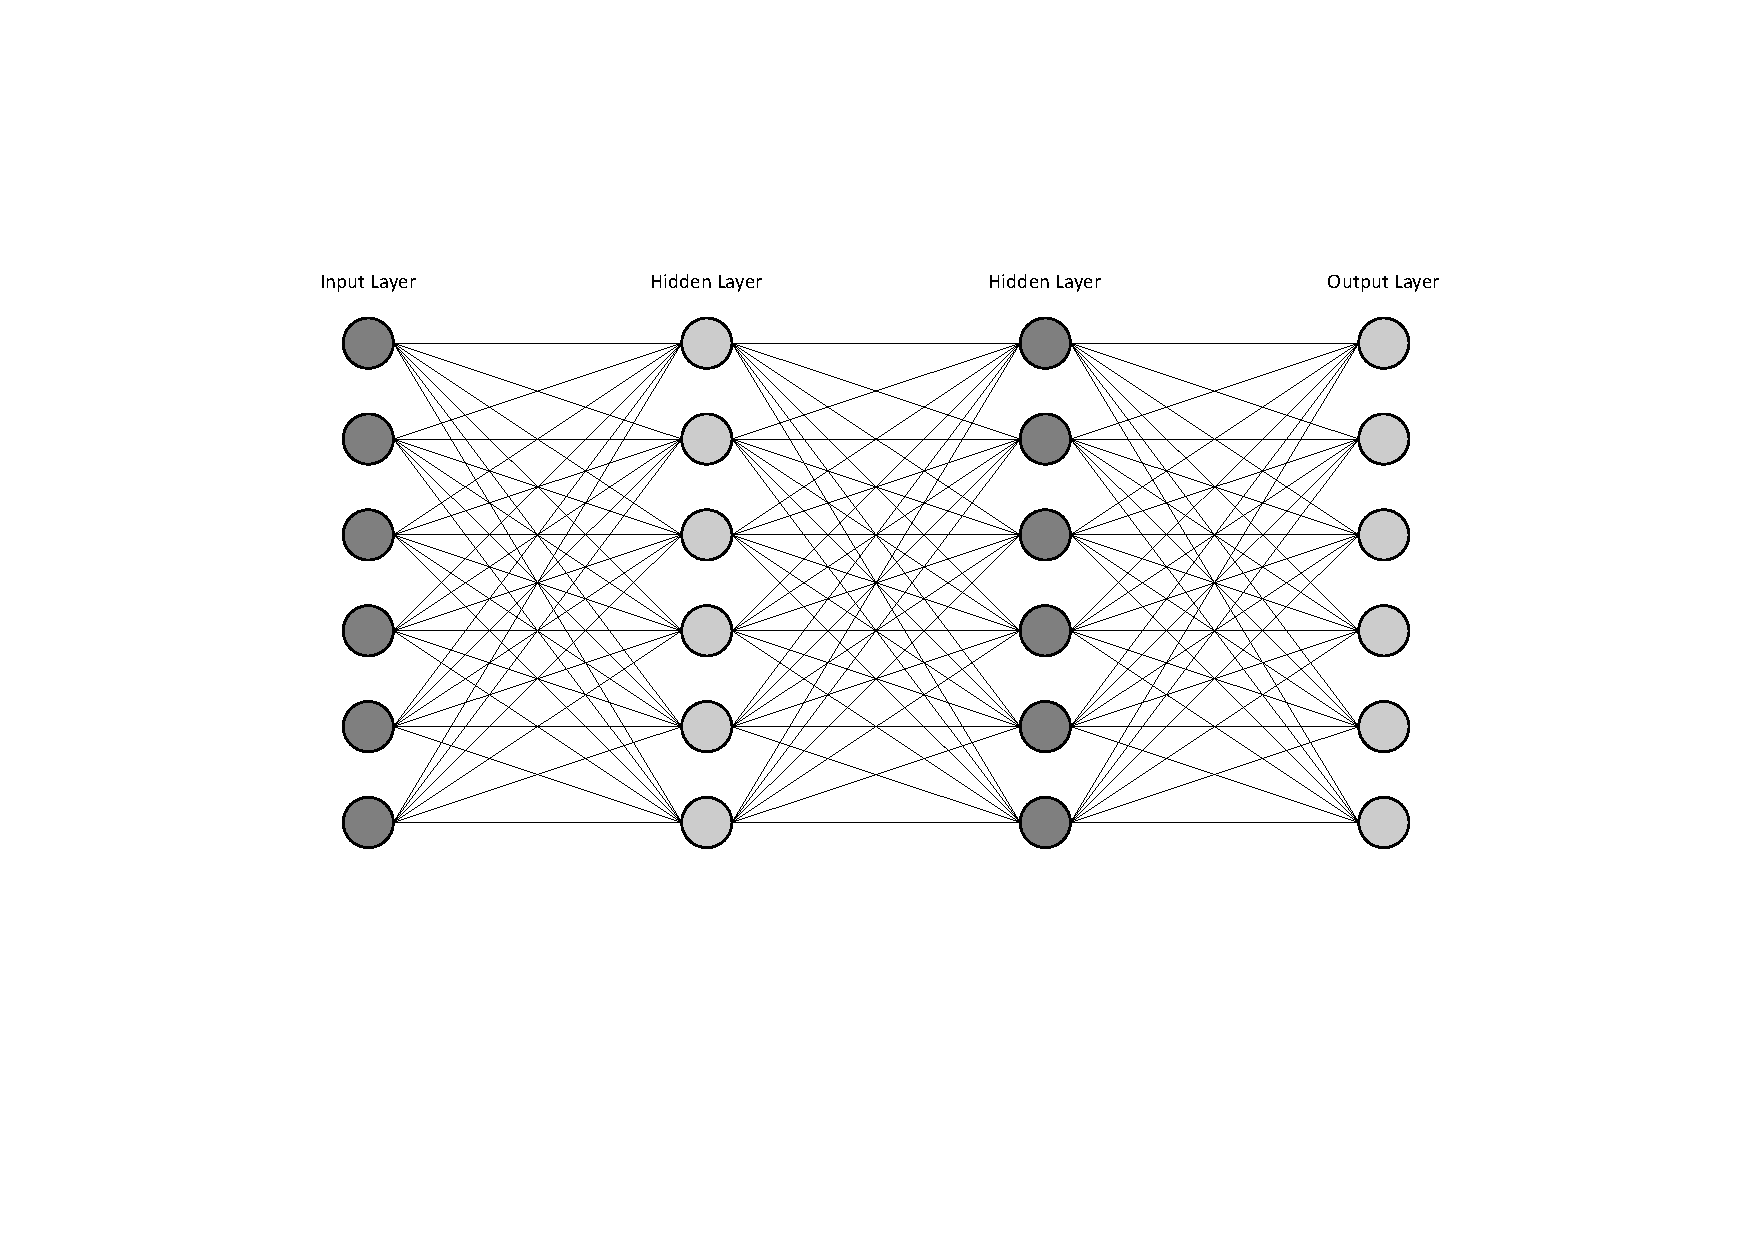
\includegraphics[width=0.7\textwidth, angle =-90]{neural_network_overview.pdf}
  \caption {Layer overview neural network}
  \label{fig:neural_network_overview}
\end{figure}

The input of a neuron is calculated from the sum of all previous neuron's outputs and one bias. Afterwards an activation function is applied to give the neural network a non-linear property. Standard multilayer feedforward networks with even one single hidden layer and an arbitrary bounded and non-constant activation function are universal approximators. This means that a wide variety of functions can be represented by the neural network when given appropriate weights \cite{HORNIK1991}. Without activation functions neural network could only make linear assignments of inputs x to outputs y. With rising data complexity the demand for a "non-linear" mapping from x to y is increasing. Without a non-linearity the neural network with several hidden layers can just learn the same functions as those with just one hidden layer. Such a neural network would not be able to mathematically realise complex relationships in the data. Fig. \ref{fig:neural_network_optimization} shows the forward- and backwardpropagation in a neural network at the example of one single neuron. First the outputs of the neurons $i$ from the previous layers $l-1$ which are connected with the neuron of interest $j$ in layer $l$ are summed up together with a bias $b_{j}$. The resulting logits $z_{j}$ are then processed by the activation function $\phi$. Different activation functions can be used throughout the network. After passing several consecutive hidden layers a loss function evaluates the prediction with the ground truth label in the end of the network.

\subsection{Activation Function}
Different problems and network layers require different activation functions. Typical activation functions are tanh, sigmoid and ReLU in the hidden as well as linear, logistic (sigmoid) and softmax in the final layers of the network \cite{Brownlee2021}. Linear final layers are used for regression problems, whereas sigmoid and softmax functions are typical for classification problems. The sigmoid function is used for binary and softmax for multiclass classification. In general the softmax function is an extension of the sigmoid function to the multiclass case, which can be proofed easily. The softmax and sigmoid functions normalize the network output to a probability distribution over the predicted output classes.  Deciding for the activation functions in the hidden layers is a little more difficult. All just mentioned functions have different characteristics which lead to individual advantages and disadvantages. The sigmoid and tanh function look pretty similar. Both squeeze the inputs in values between -1 and 1. Both functions can suffer from the vanishing gradient problem since the derivative of these functions is close to zero for very big or small inputs. A solution for that is the ReLU function which solves that problem but is limited due to the mapping of negative inputs to zero (dead ReLU) \cite{Brownlee2021}. In table \ref{tab:activation_functions} some of the most popular activation functions are described. \newline
\newline



\begin{tabular}{ c c c c }
\hline 
Formula & Formulation s(x) & Derivative $\frac{ds(x)}{dx}$ & Function output range \\ \hline                        
ReLU &   \begin{cases} 0 & \text{, for }x < 0\\
	x & \text{, for }x \geqslant 0 \end{cases} & \begin{cases} 0 & \text{, for }1 < 0\\
	1 & \text{, for }x \geqslant 0 \end{cases} & [ 0, \infty)\\

\rule{0pt}{5ex}%  EXTRA vertical height 

Leaky ReLU &   \begin{cases} \alpha x & \text{, for }x < 0\\
	x & \text{, for }x \geqslant 0 \end{cases} & \begin{cases} \alpha & \text{, for }1 < 0\\
	1 & \text{, for }x \geqslant 0 \end{cases} & (-- \infty, \infty)\\

\rule{0pt}{5ex}%  EXTRA vertical height 

ELU &   \begin{cases} \alpha(e^{x} - 1) & \text{, for }x < 0\\
	x & \text{, for }x \geqslant 0 \end{cases} & \begin{cases} \alpha e^{x} & \text{, for }x < 0\\
	1 & \text{, for }x \geqslant 0 \end{cases} & [−\alpha, \infty)\\
	
\rule{0pt}{5ex}%  EXTRA vertical height 
	
Sigmoid & $\frac{1}{1+e^{-x}}$ & $\frac{e^{-x}}{(1+e^{-x})^{2}}$ & (0,1)\\

\rule{0pt}{5ex}%  EXTRA vertical height 

Softmax & $\frac{e^{x_{i}}}{\sum_{j=1}^{K} e^{x_{j}}}$ & $\frac{e^{-x}}{(1+e^{-x})^{2}}$ & (0,1)\\

\rule{0pt}{5ex}%  EXTRA vertical height 

tanh & $\frac{e^{2x}-1}{e^{2x}+1}$ & $1-tanh^{2}(x)$ & (-1,1) \\
\hline  
\label{tab:activation_functions}

\end{tabular}
\captionof{table}{Overview activation functions}




\subsection{Optimization}
When training neural networks one has to decide for a loss function and an optimizer. 

\subsubsection{Loss}
The loss function acts as a model evaluation criterion and the optimizer is responsible for adapting the model accordingly. Deep Learning models can be divided into two groups: (1) regression tasks and (2) classification tasks. In a regression problem the goal is to learn a mapping function from input variables to a continuous output variable. Contrairwise, in a classification problem the model aims to predict the class label from the input variables \cite{ShilohPerl2020}. Typically Mean Square Error (MSE) , shown in eq. \ref{eq:MSE} , is used for regression problems:

\begin{equation}
L(X) =  \sum_{x}(\hat{y}(x)-y(x))^2
\label{eq:MSE}
\end{equation}

where $y(x)$ is the ground truth and $\hat{y}(x)$ the predicted class label \cite{ShilohPerl2020}. The Cross Entropy Loss, shown in eq. \ref{eq:CE} is rather more used for classification problems: 

\begin{equation}
L(X) = \sum_{x} y(x) log(p(x))
\label{eq:CE}
\end{equation}
where p(x) is the predicted probability of the sample $x$ belonging to the ground truth class $y(x)$ \cite{ShilohPerl2020}.

\subsection{Training Loop}
The weights and biases of the model are adapted such that the loss is minimized. This optimization takes place in a two stage process: (a) feed-forward pass of the input data throughout the model and calculating corresponding neuron outputs and the loss from the predicted and ground-truth labels; followed by (b) backward pass of the loss throughout the model and updating the model weights accordingly. Iteratively this process is performed to optimize the model performance. During the backward pass the gradients of the loss with respect to the network weights is calculated and used to update the weights and biases of the network. The process is visualized in fig. \ref{fig:neural_network_optimization} (green: forward pass, red: backward pass). All the weights and biases are updated recursively by calculating the gradients of every layer, starting from the final and ending at the input layer. Using the chain rule, different partial derivatives of the network can be concatenated. Eq. \ref{chain_rule} shows the chain rule used during backpropagation:
\begin{equation}
 \frac{\delta L_{i}}{\delta w_{i}} = \frac{\delta L_{i}}{\delta \hat{y_{i}}} * \frac{\delta \hat{y_{i}}}{\delta z_{i}} * \frac{\delta z_{i}}{\delta w_{i}}, 
 \label{chain_rule}
\end{equation}
where $\frac{\delta L_{i}}{\delta \hat{y_{i}}}$ is the derivative of the loss with respect to the output of the activation function of the last layer, $\frac{\delta \hat{y_{i}}}{\delta z_{i}}$ is the derivative of the activation function and $\frac{\delta z_{i}}{\delta w_{i}}$ is the derivative of the logits $z_{i}$ with respect to the weights and biases \cite{ShilohPerl2020}.

\begin{figure}[htpb]
  \centering
  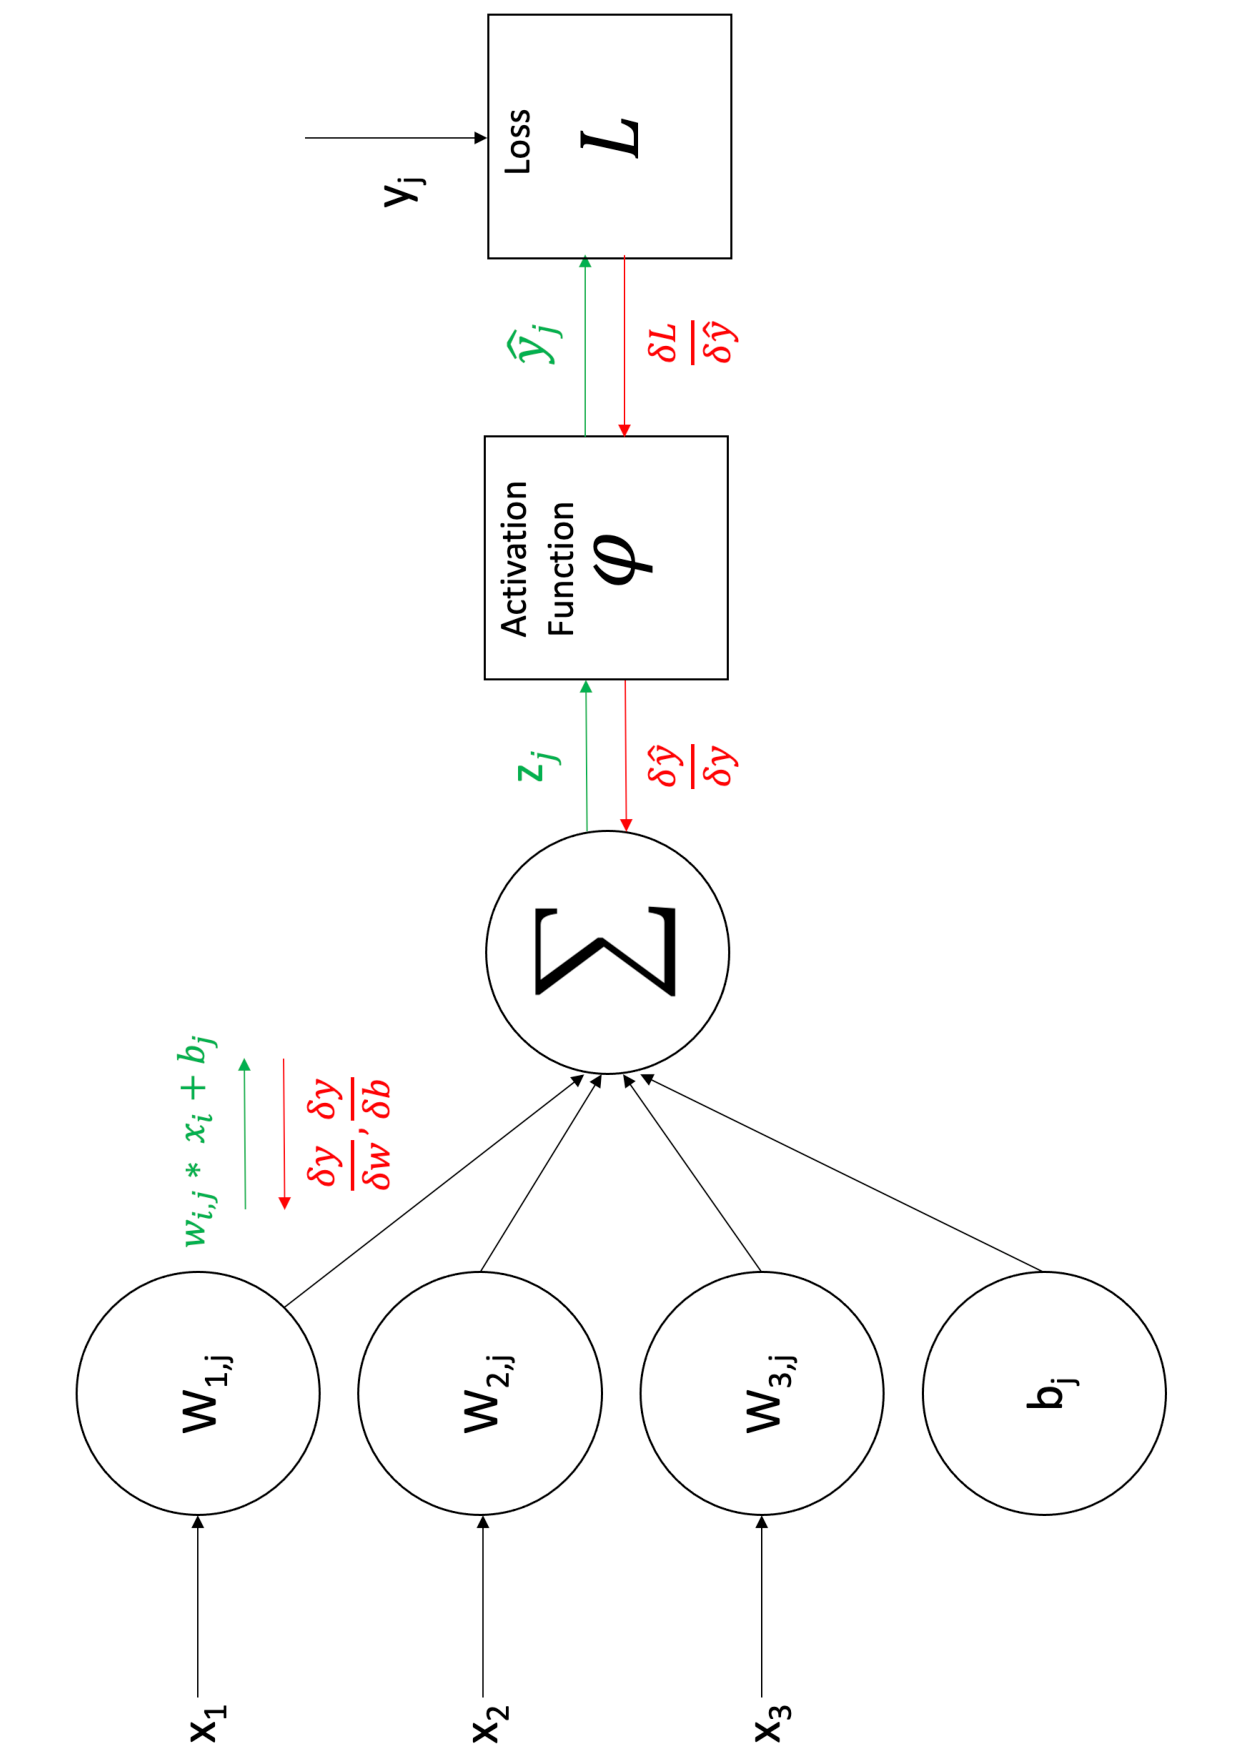
\includegraphics[width=0.7\textwidth, angle = -90]{neural_network_optimization.pdf}
  \caption {Optimization of neural network}
  \label{fig:neural_network_optimization}
\end{figure}


\subsection{Optimizer}
Calculating the gradient for the whole dataset is computationally expensive. A common practice is therefore to separate the dataset in several subsets, so called mini-batches. For each mini-batch the corresponding gradients are calculated and the model is updated accordingly. This process is repeated for all the mini-batches retrieved from the dataset. Each cycle of training over the whole dataset is called an epoch and in every cycle. When the loss converges the training can be terminated. Despite convergence an optimal solution is not assured since the most neural network problems are not convex \cite{ShilohPerl2020}.


Applying gradient descent based optimizer, the weights and biases are updated with a step in the negative direction of the derivative:

\begin{equation}
  w_{new} = w_{old} - \eta \frac{\delta L}{\delta w_{old}},
\end{equation}
where $w_{old}$ are the old, $w_{new}$ are the new model parameters, $\eta$ is the learning rate and $\frac{\delta L}{\delta w_{old}}$ is the derivative of the loss with respect to the current model weights \cite{ShilohPerl2020}. 
Most optimizer rely only on the gradients (first order methods). Using second-order methods do generally converge faster but also require the computation of the Hessian. This is especially expansive for big datasets and models. For this reason Stochastic Gradient Descent is an optimization option which randomly picks samples to optimize the model. For this reason Stochastic Gradient Descent (SGD) is used, which calculates the gradient for single randomly picked samples from the dataset. Since the choice of these samples is random, the optimization suffers from instability and fluctuation. Instead of regular SGD one can use mini-batch gradient descent. This is a compromise between the regular SGD and gradient descent method. The gradient and model update is neither performed for a single sample nor for the whole dataset, but it is performed on a small randomly picked subset of the dataset, which accelerates the convergence of the training.\newline
\newline
\textbf{Momentum}\newline
In order to accelerate and stabilize the optimization one can also include historical gradients. First and second Momentum is a method that helps accelerate SGD in the relevant direction and dampens oscillations \cite{ShilohPerl2020} . Instead of updating with a fixed stepsize in the direction of the negative gradient one can use first and second momentum to adapt the stepsize of the optimization in the different dimensions. In the following four different optimizer which use first, second momentum or a combination of those. An optimization with first momentum works as follows:

\begin{equation}
  \begin{aligned}
  v_{t} = & \gamma v_{t-1} +  \eta \nabla_{\theta}L(W_{t-1}) &\\
  W_{t} = &W_{t-1} - v_{t},
  \end{aligned}
  \label{eq:moment}
\end{equation}

where $M_{t}$ is the momentum, which calculates a moving average over the past gradients, $\nabla_{\theta}L(W_{t})$ is the derivative of the loss with respect to the current model weights, $\beta$ defines the relationship between current gradient and momentum in the moving average, $W_{t-1}$ are the current and $W_{t}$ the updated model weights \cite{Ruder2016}.\newline
\newline
\textbf{Nesterov accelerated gradient (NAG)}\newline
Another well known optimizer of this kind is NAG which works just like described in  \ref{eq:moment}. The only difference is that that the gradient is not estimated for the current, but for some pre-udpated model weights. In a first step the gradient is calculated for the old model weights, which are updated with the momentum from the previous iteration $\nabla_{\theta}L( W_{t-1} - \gamma v_{t-1})$. In a second step the current model weights  are updated with the moving average of the momentum and gradient as described in \label{eq:moment} \cite{Ruder2016}.\newline
\newline
\textbf{Adagrad}\newline
Instead of using first momentum, Adagrad builds a moving average of the the past squared gradients (second momentum):

\begin{equation}
  \begin{aligned}
  W_{t} = W_{t-1} - \frac{\eta}{\sqrt[2]{G_{t}+ \epsilon}} \bigodot \nabla_{\theta}L(W_{t-1}),
  \end{aligned}
  \label{eq:Adagrad}
\end{equation}

where  $W_{t-1}$ are the current and $W_{t}$ the updated model weights, $\nabla_{\theta}L(W_{t})$ is the derivative of the loss with respect to the current model weights, $G_{t}$ is second momentum and $\epsilon$ denotes a small quantity which prevents the division by zero  \cite{Ruder2016}.\newline
\newline
\textbf{Adaptive Moment Estimation (ADAM)}\newline
The Adam is one of the most popular optimizer. ADAM combines the idea of first and second momentum: 
\begin{equation}
  \begin{aligned}
   &m_{t} =  \beta_{1} m_{t-1} +  (1-\beta_{1}) \nabla_{\theta}L(W_{t-1}) &\\
    &v_{t} =  \beta_{2} v_{t-1} +  (1-\beta_{2}) \nabla_{\theta}L^{2}(W_{t-1}) &\\
    &\hat{m}_{t} = \frac{m_{t}}{1-\beta_{1}^{t}}&\\
    &\hat{v}_{t} = \frac{v_{t}}{1-\beta_{2}^{t}}&\\
   & W_{t} = W_{t-1} - \frac{\eta}{\sqrt[2]{\hat{v}_{t} + \epsilon}}\hat{m}_{t}, &\\
  \end{aligned}
  \label{eq:moment}
\end{equation}

where $m_{t}$ and $v_{t}$ are the first and second momentum, $\hat{m}_{t}$ and $\hat{v}_{t}$ are the bias-corrected first and second moment estimates, $\beta_{1}$ and $\beta_{2}$ are the weighting factors for the moving average and $W_{t-1}$ and  $W_{t}$ are the current and updated model weights \cite{Ruder2016}.



\section{Convolutional Neural Network (CNN)}

Equally to regular neural networks CNNs consist of several neurons embedded in a fixed architecture. CNNs focus on processing images and therefore the architecture is set up such that dealing with images is optimized. In CNNs the neurons are structured in layers just like in normal neural networks. In regular networks the neurons of one layer are are organized in one dimension and in CNNs in three dimensions (height, width, depth).

The functionality of CNNs are visualized in \ref{fig:CNN_overview}. One can identify four main compounts of a CNN, which are described more detailed in the following:

\begin{itemize}
    \item [1.] Data which is organized in a structured 1D or 2D form is fed into the CNN as input layer. Each element in this structure is called a pixel. A pixel contains a specific value and position in the structure. 
    
    \item [2.] The convolutional layer contains kernels which are convolved with the input. The kernels contain weights and biases which are learned during training. The rectified linear unit (ReLu) aims to apply as an ’elementwise’ activation function to the kernel outputs.
    
    \item [3.] The pooling layer downsamples along the spatial dimensionality. This reduces the size of the feature maps which are fed through the network in order to minimize the learnable parameters in the network.
    
    \item [4.] In the end fully-connected layers attempt to predict a class label for each input sample. Also Relu can be used as activation functions in these layers.
\end{itemize}

\begin{figure}[htpb]
  \centering
  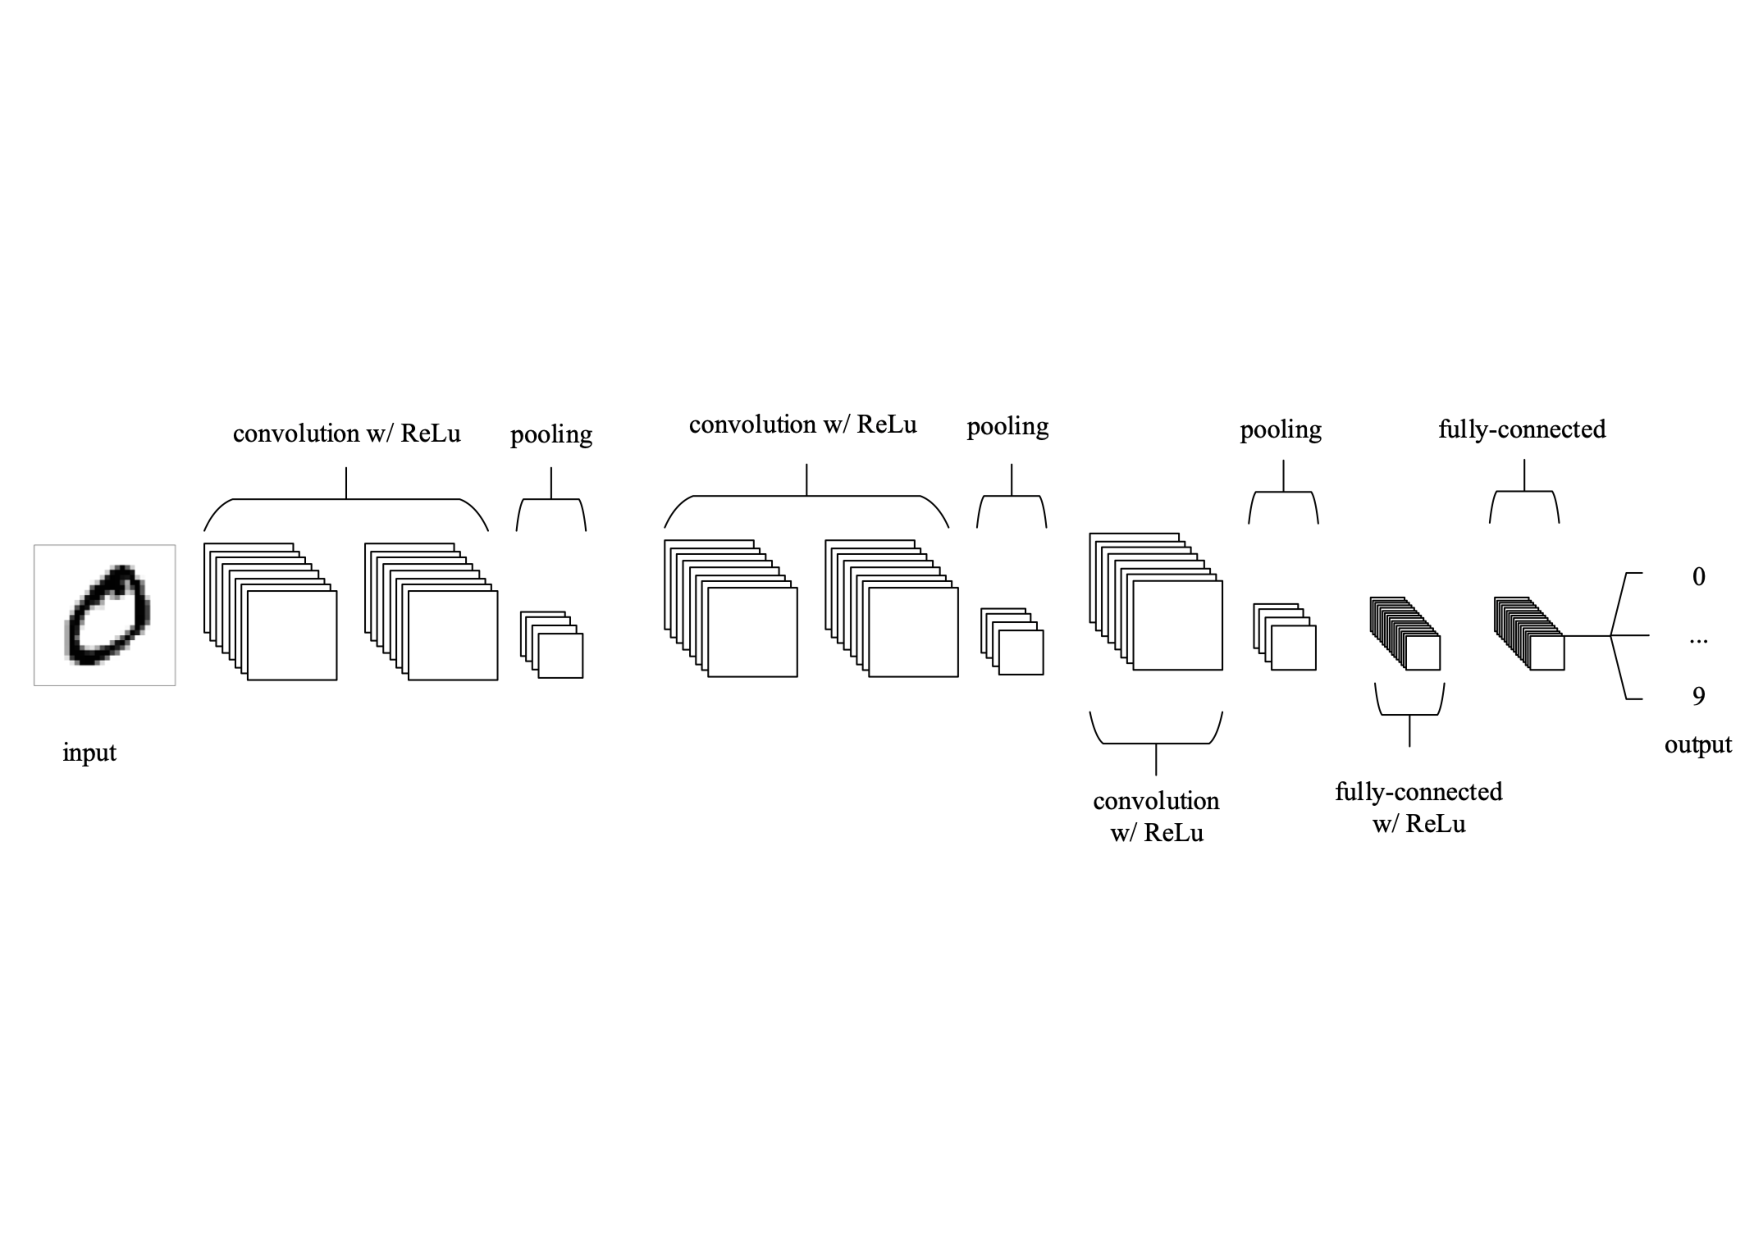
\includegraphics[width=0.9\textwidth]{cnn/cnn_architecture.pdf}
  \caption {Overview over CNN architecture \cite{OShea2015}}
  \label{fig:CNN_overview}
\end{figure}
Besides operations like Batch-Normalization, which are also common in regular neural networks, CNNs apply pooling layers. Pooling layers are responsible for downsampling the feature maps along the spatial dimensionality to reduce the complexity of the model. In the following typical CNN layers are described more in detail. 


\subsubsection{Kernels}
The convolutional layers are the core layers of a CNN. The learnable paramaters in a convolutional layer are the weights and biases of each kernel. During the optimization each kernel learns to extract expressive features. Usually the spartial dimensions (width, height) are reduced throughout the network in order to go from extracting global features in the beginning to more local features in the end. Since the kernels are applied at different regions of the input the kernel scans different locations for the learned features. The depth of a kernel is defined by the depth of the input. Each kernel produces a feature map of depth one. It is possible to apply several equal kernels such that the total depth of the feature map is increased. Each channel corresponds to the features extracted by one single kernel \cite{OShea2015}. Looking at fig. \label{fig:kernel_number} one can see how the kernel of depth 3 (orange) is applied on the input of depth 3 (blue). By using 128 kernels the resulting feature map is of depth 128.

\begin{figure}[htpb]
  \centering
  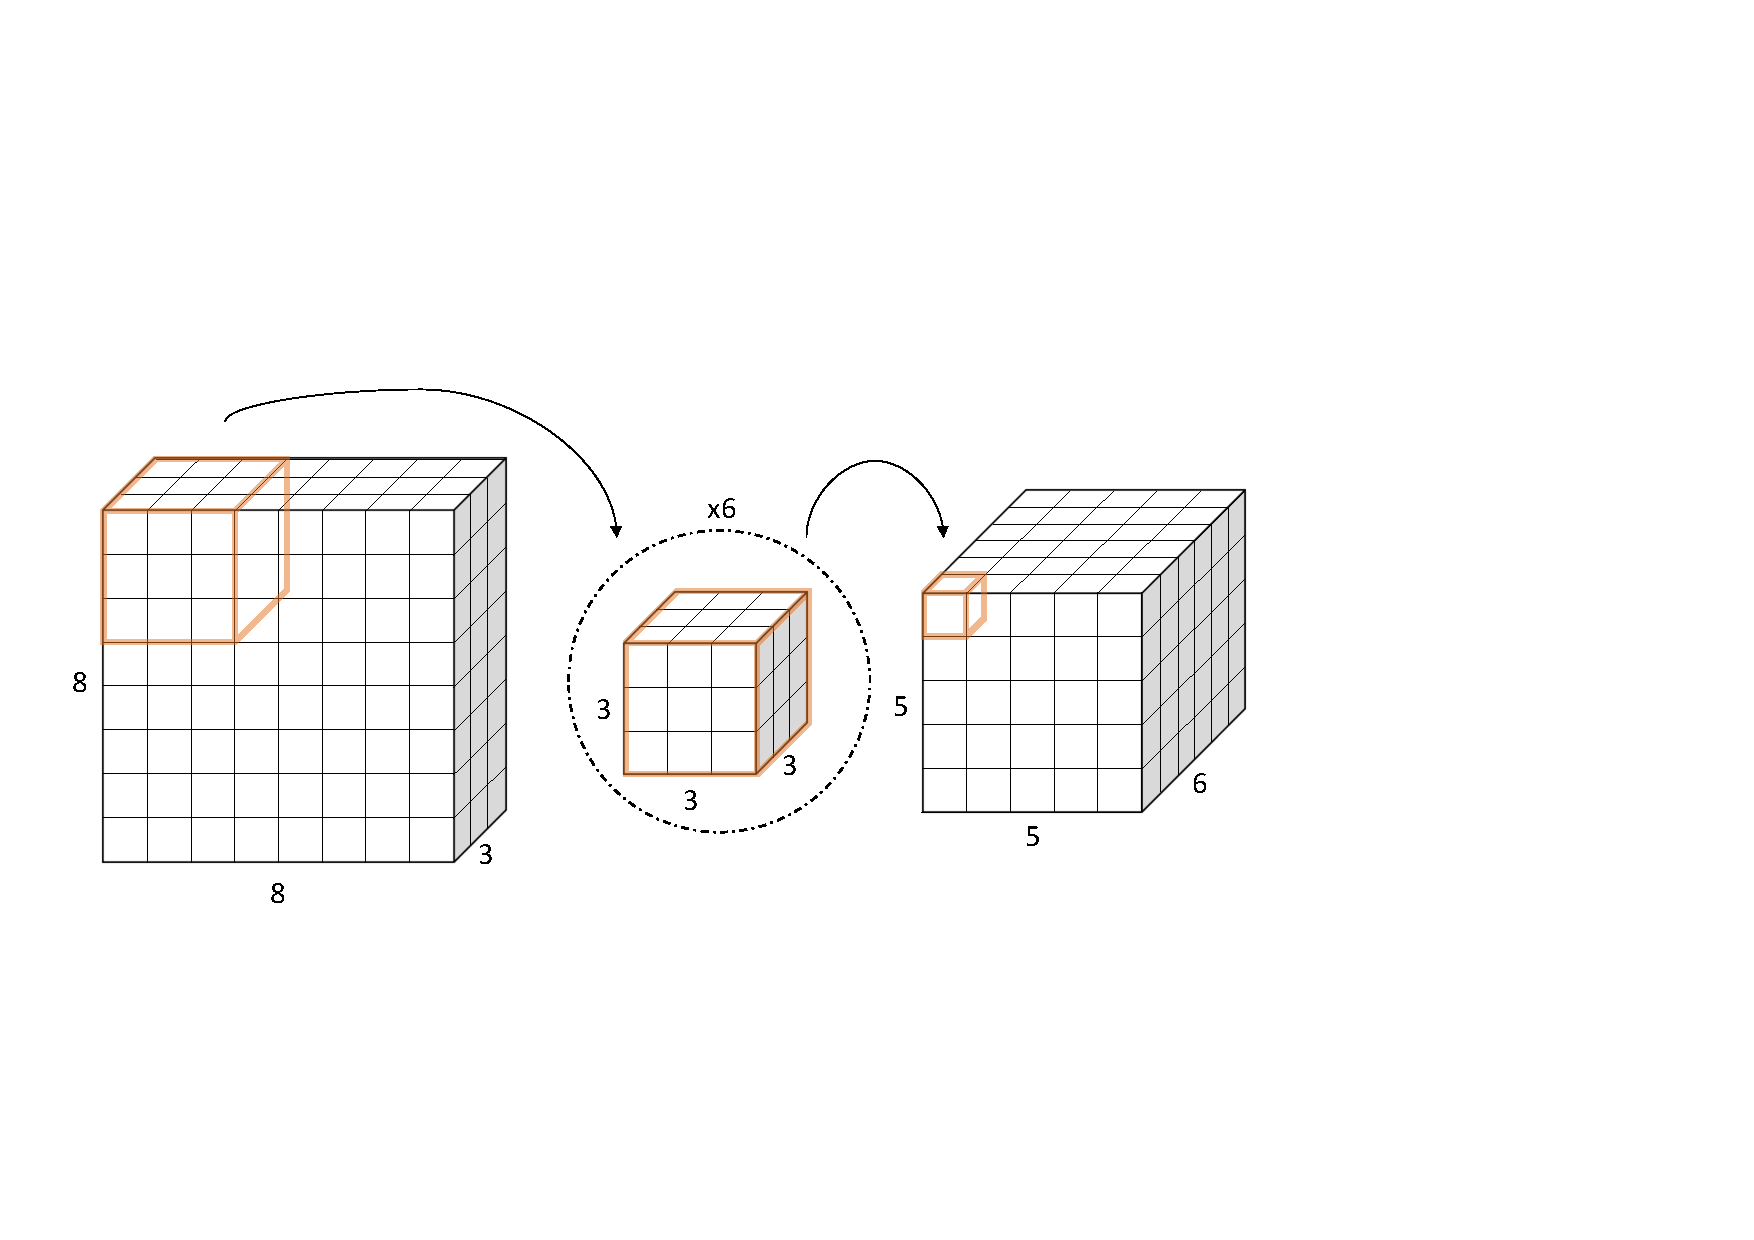
\includegraphics[width=0.6\textwidth]{cnn/kernel_number.pdf}
  \caption {2D convolution with 128 kernels of depth 3 \cite{Ganesh2019}}
  \label{fig:kernel_number}
\end{figure}
\FloatBarrier 

In a convolutional layer each kernel is convolved with the data across the whole spatial dimensionality. A feature map of new spatial dimension is created \cite{OShea2015}. To make things easier the convolution is shown for the 1D case:

\begin{equation}
  y(p_{0}) = \sum_{p_{n} \in R} w(p_{n}) \cdot x(p_{0} + p_{n}), 
  \label{eq:kernel}
\end{equation}

where $p_{n}$ is one of the $R$ cells in the kernel, $p_{0}$ is the starting pixel of the input. Each kernel cell is multiplied with the corresponding pixel in the input and the $R$ outputs are summed up in the pixel $p_{0}$ of the feature map \cite{Ganesh2019}. This process is also visualized in fig. \ref{fig:kernel}, where $p_{n}$ is one of the three cells within the kernel, $R$ is three in this case and $p_{0}$ marks the the position of the convolution in the input and feature map. In this case $p_{0}$ is two since the first pixel of the input is not used and the second pixel in the feature map is calculated.


\begin{figure}[htpb]
  \centering
  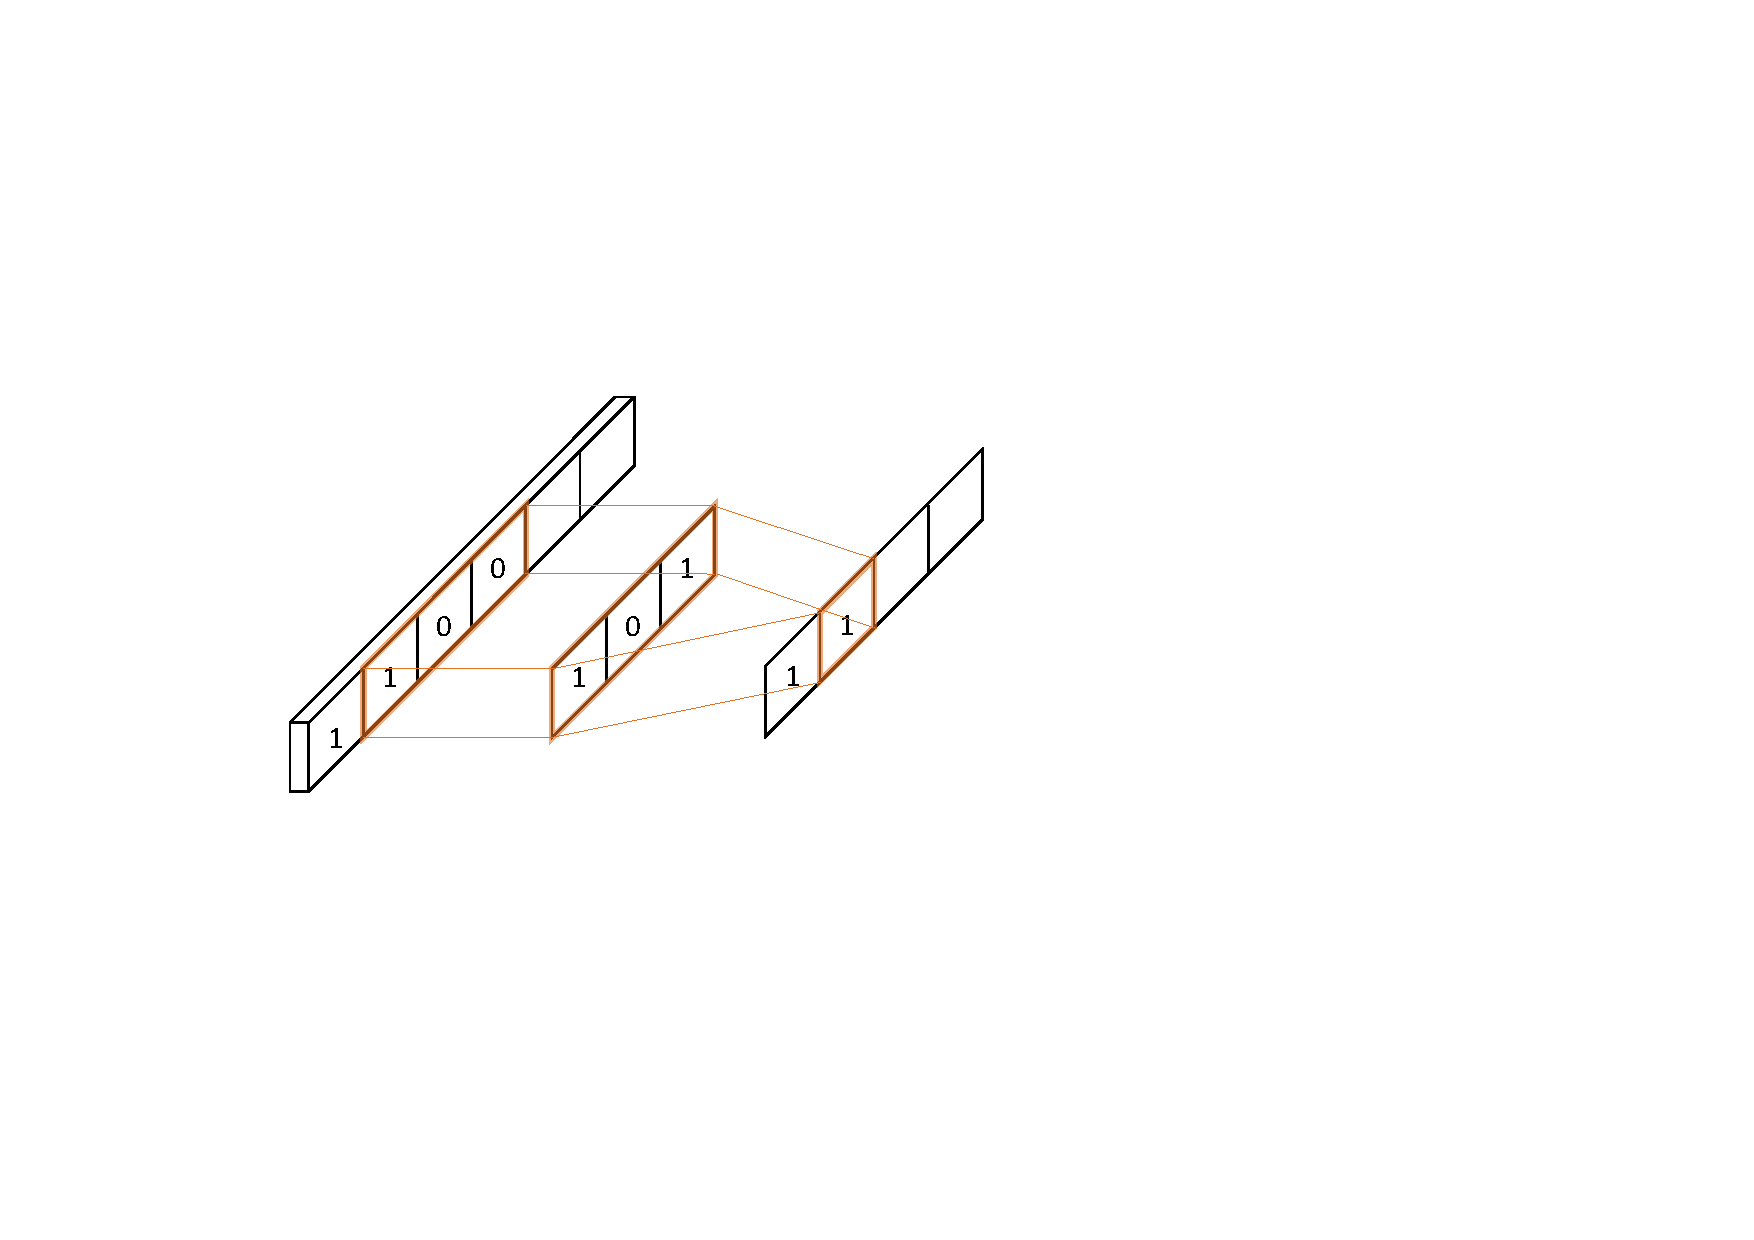
\includegraphics[width=0.5\textwidth]{cnn/kernel_calculation.pdf}
  \caption {Convolution of kernel an input \cite{Ganesh2019}}
  \label{fig:kernel}
\end{figure}

Compared to regular neural networks CNNs profit a lot from it's weight sharing concept. The kernel weights are learned throughout the training. Since the kernel is applied on different parts of the input, it is not necessary to train a weight for each input pixel. This reduces the number of learnable parameters in the network \cite{OShea2015}. Since the kernel is applied on different input locations, the feature search is insensitive to feature location in the image.

\subsubsection{Dilated convolution}

The dimensionality of the input which is processed by the kernel is called receptive field. When increasing the receptive field more global and otherwise more local features of the input are extracted. When defining a CNN architecture one has to find a trade-off between a model which is complex enough to capture the important information from the data and also keep the number of parameters low. Several hyperparameters can be used to reduce or increase the complexity of the model. After a convolutional layer three hyperparameters can be used to define the width and height of the resulting feature map. Dilated convolution, shwon in fig.\ref{fig:dilated_cnn}, is the same as regular convolution but it involves pixel skipping, so as to cover a larger area of the input. The kernel is not applied on a every neighbouring pixel \cite{Ganesh2019}.

\begin{figure}[htpb!]
  \centering
  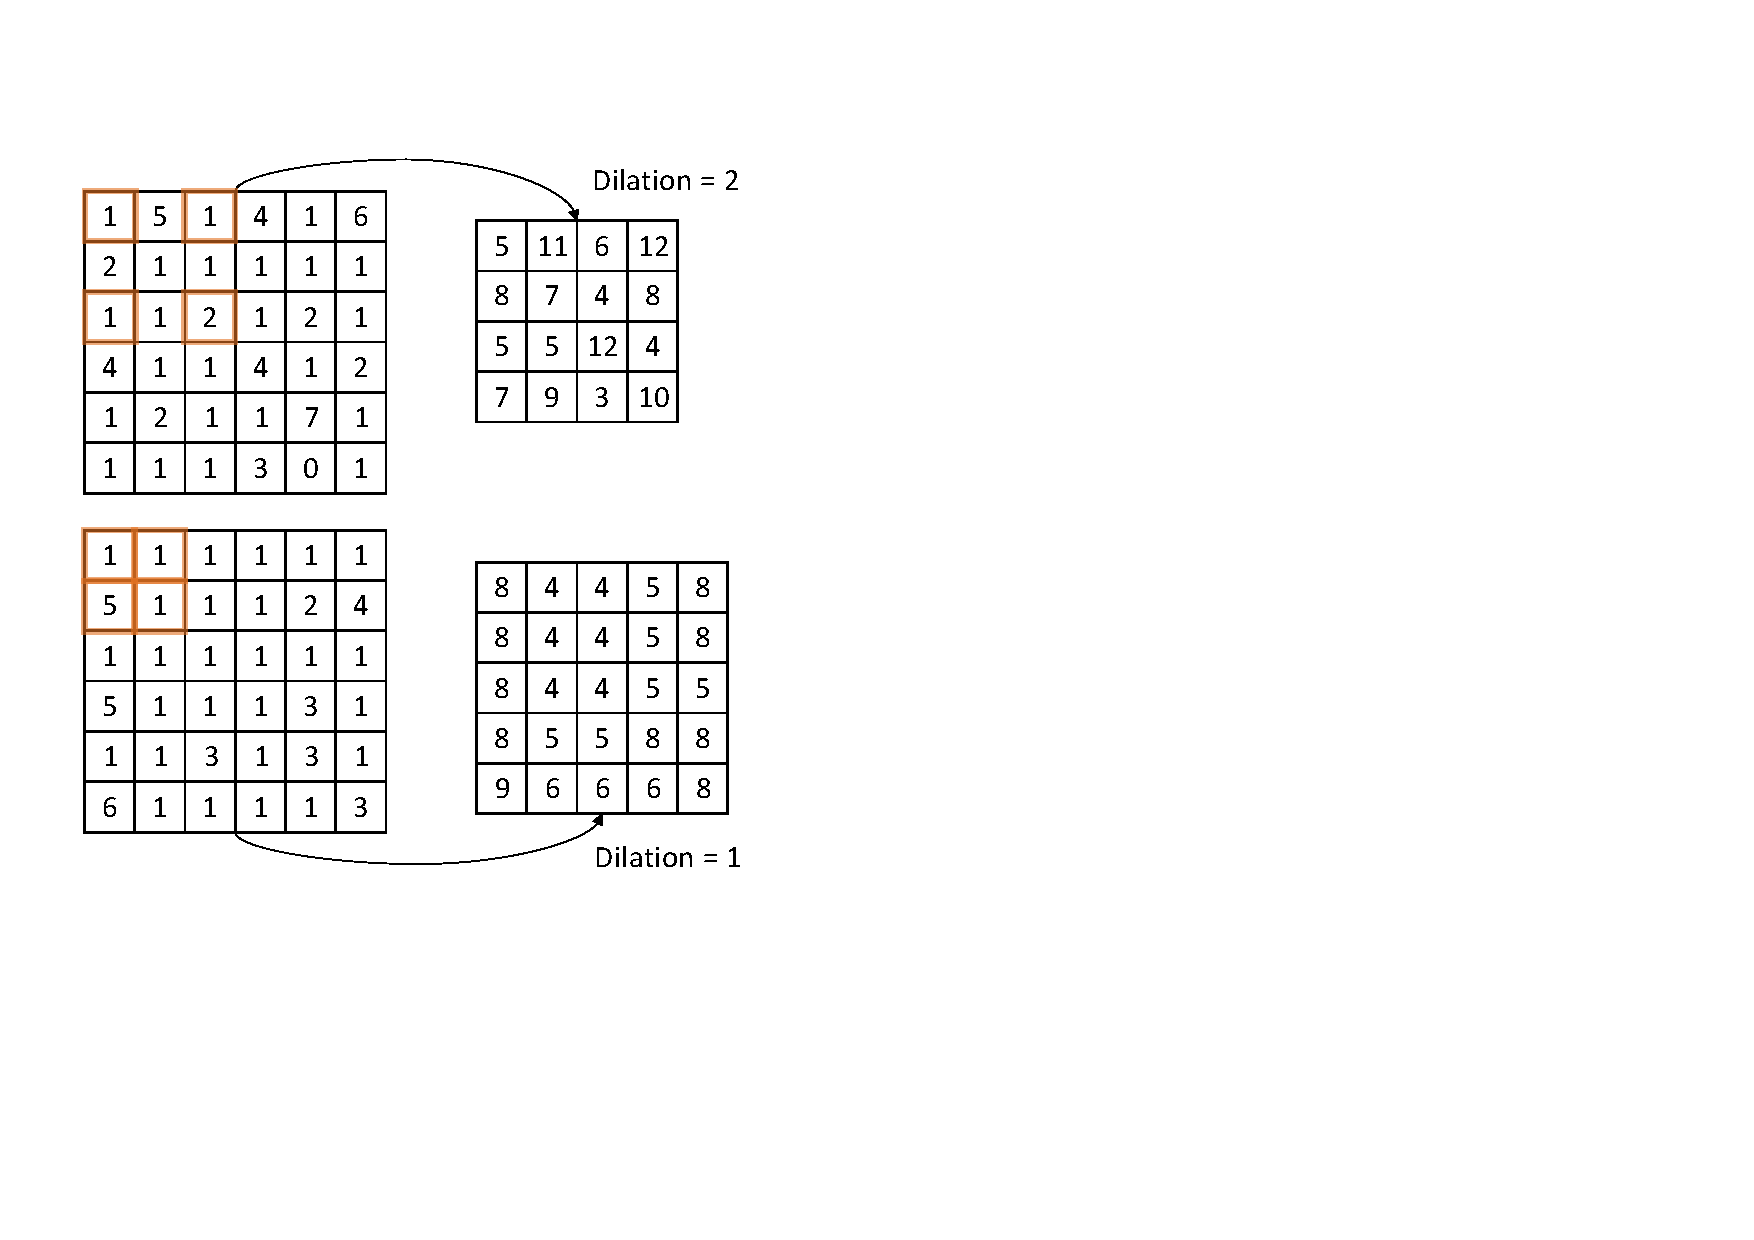
\includegraphics[width=0.5\textwidth]{cnn/dilation_cnn.pdf}
  \caption {Receptive field for convolution with different dilation factors}
  \label{fig:dilated_cnn}
\end{figure}
\FloatBarrier 

\subsubsection{Stride}
By increasing the stride the kernel skips several pixels while shifting over the input. The effects of an different stride factors are shown in fig.\ref{fig:stride_cnn}. The resulting feature map is decreased with an increased stride factor \cite{OShea2015}.

\begin{figure}[htpb]
  \centering
  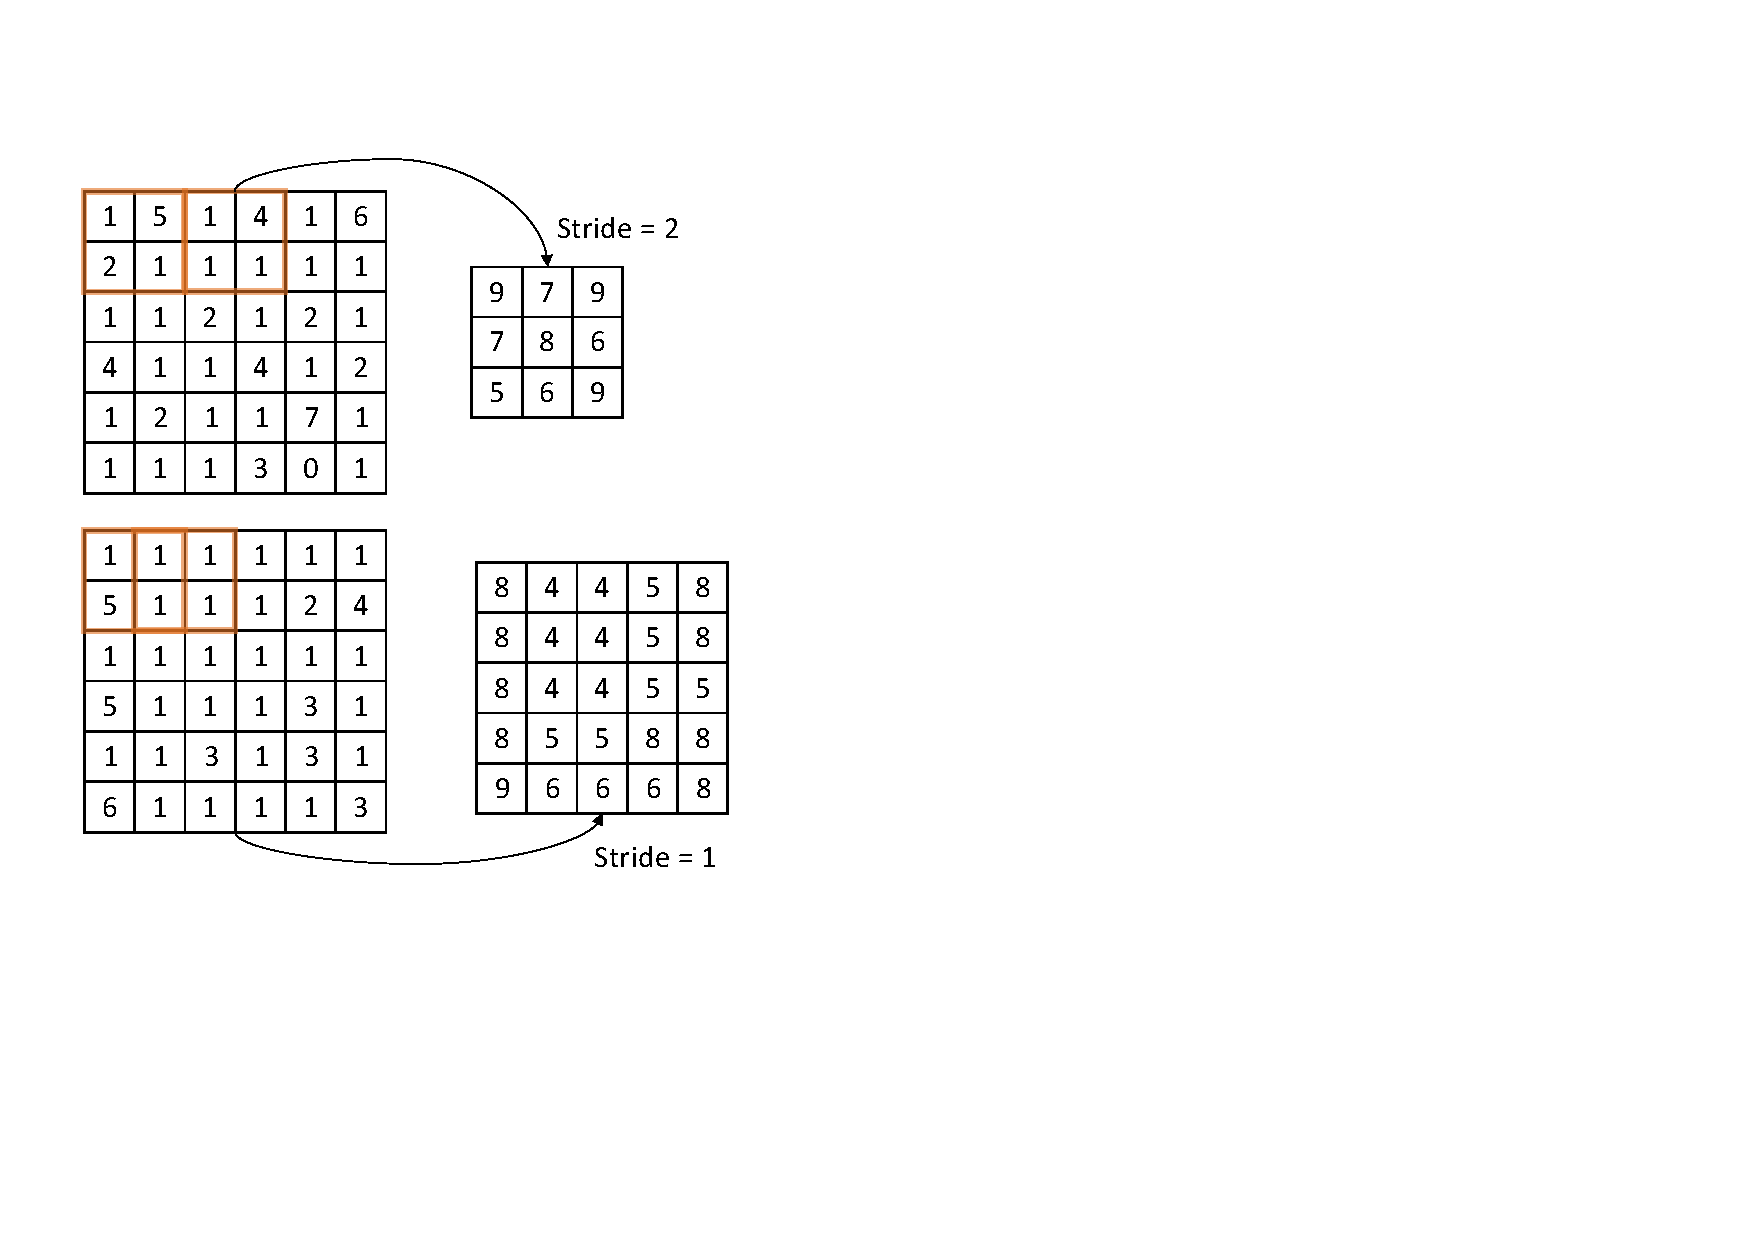
\includegraphics[width=0.5\textwidth]{cnn/stride_cnn.pdf}
  \caption {Convolution with different stride factors}
  \label{fig:stride_cnn}
\end{figure}
\FloatBarrier 

\subsubsection{Zero padding}
Zero padding, shown in fig.\ref{fig:zero_padding_cnn}, enlarges the input with a border of zeros, which increases the resulting feature map \cite{OShea2015}.

\begin{figure}[htpb]
  \centering
  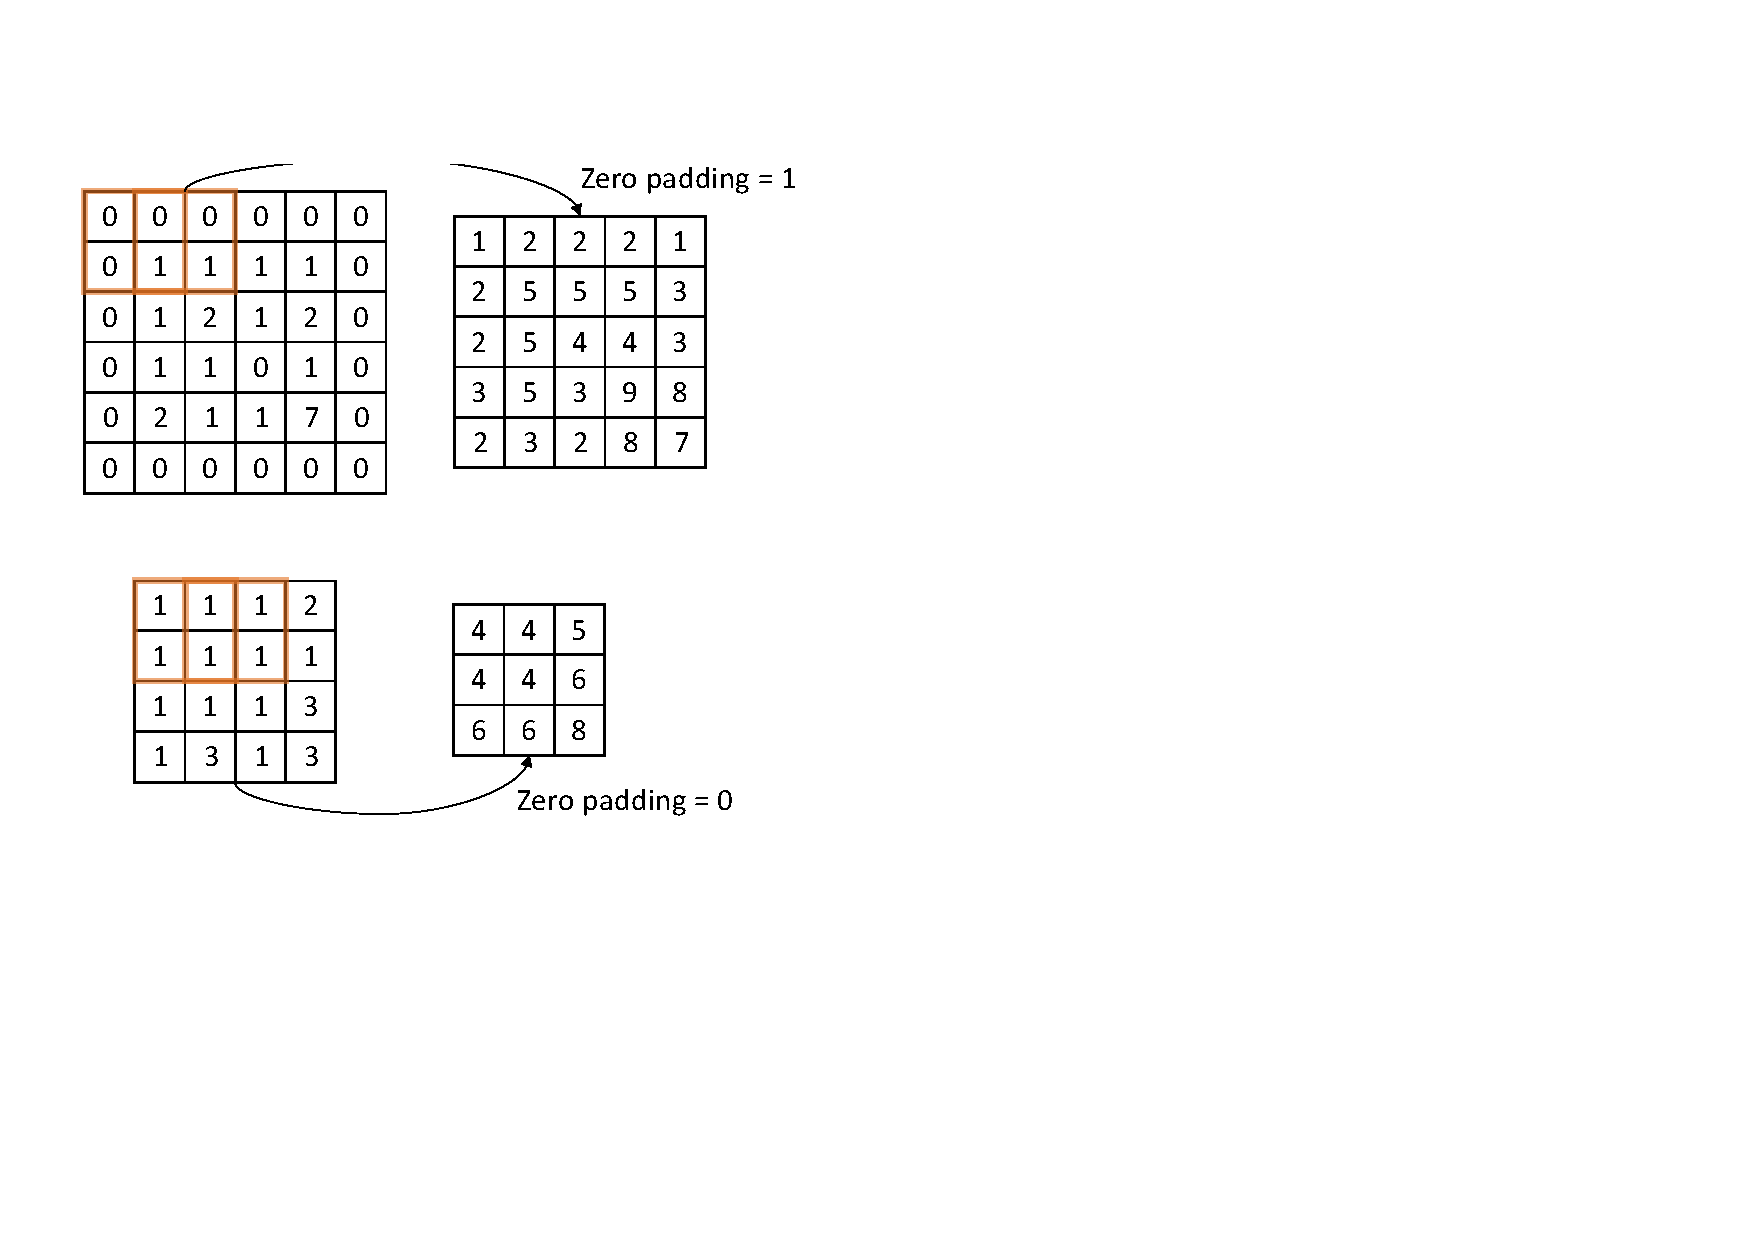
\includegraphics[width=0.5\textwidth]{cnn/zero_padding_cnn.pdf}
  \caption {Convolution with different zero padding}
  \label{fig:zero_padding_cnn}
\end{figure}
\FloatBarrier 


\subsubsection{Spatial dimensionality}

 The spatial dimensionality of the feature map right after a convolutional layer can be calculated as follows:

\begin{equation}
  \frac{(V-R)+2Z}{S+1}, 
  \label{eq:spatial_dimensionality_cnn_feature map}
\end{equation}
where V is the input size, R is the size of the receptive field, Z is the amount of zero padding and S refers to the stride.

\subsubsection{Pooling layer}
To change the spatial dimensionality of the data feed through the network one can also include pooling layers. There exist different variants like max-pooling and average pooling. In general these layers work identical as convolutional layers just that they do not have learnable parameters. Also pooling kernels are shifted over the input. For each kernel position all pixels covered by the kernel are merged to a single value. Max-pooling returns the maximal pixel value and average-pooling the average over all pixels. Often convolutional and pooling layers are applied consecutively \cite{OShea2015}.

\section{Generative Adversarial Networks (GAN)}
GANs are generative models which recently became more and more popular. Generative models can capture the data distribution of the samples seen during training. Such models are able to generate new instances which belong to the learned distribution but are not actually part of it. GANs inlcude two different models. A generator network (G) learns the data distribution of the training data. Given noise the generator network produces synthetic data. The discriminator (D) model tries to classify the seen data between the synthetic generator's output and the true data. D(x) represents the probability that x came from the real data rather than from the generator. The optimization process of GANs is a minimax game process:
\begin{equation}
    \min_{G} \max_{D} \mathbb{E}_{x \sim P_{r}} [log(D(\tilde{x}))] + \mathbb{E}_{x \sim P_{g}}[log(1-D(\tilde{x}))],
    \label{eq:GAN_Training}
\end{equation}
where $P_{r}$ is the data distribution of real and $P_{g}$ is the data distribution from the generator, which is defined by  $\tilde{x}  \sim G(z)$ and  $z \sim p(z)$. z is sampled from a specific distribution like the Uniform or Gaussian distribution. In theory the generator should be learned such that eq. \ref{eq:GAN_Training} is minimized. This is achieved when $D(x) \sim 0$ and $D(\tilde{x}) \sim 1$, which is the case if the discriminator falsely classify the real and the synthetic generator's outputs. On the other hand, the discriminator should be learned such that eq. \ref{eq:GAN_Training} is maximized, which means that the discriminator correctly labels all samples. The discriminator and generator are optimized in an alternating procedure \cite{Goodfellow2014}. In order to prevent overfitting the one should alternate between k steps of optimizing D and one step of optimizing G \cite{Goodfellow2014}. The optimization of GANs proposed by Goodfellow et al \cite{Goodfellow2014} is described in the Algorithm \ref{alg.GAN_optimization}.

\begin{algorithm}
\caption{Iterative optimization of GANs}\label{alg:cap}
\begin{algorithmic}
\While{$\textrm{train iterations} < \textrm{max iterations}$}
    \While{$\textrm{discriminator optimization steps} < \textrm{k}$}
        \State $\cdot$ Sample m noise samples ${\pmb{z}^{(1)}, . . . , \pmb{z}^{(m)}}$ from noise distribution $p(\pmb{z})$
        \State $\cdot$ Sample m noise samples ${\pmb{x}^{(1)}, . . . , \pmb{x}^{(m)}}$ from real data distribution $P_{r}$
        \State $\cdot$ Update the discriminator by ascending its stochastic gradient:
        \begin{equation*}
            \nabla_{\theta_{d}} \frac{1}{m} \sum_{i=1}^{m} [log(D(\pmb{x}^{(i)})) + log(1-D(G(\pmb{z}^{(i)})))].
        \end{equation*}
    \EndWhile
    \State $\cdot$ Sample m noise samples ${\pmb{z}^{(1)}, . . . , \pmb{z}^{(m)}}$ from noise distribution $p(\pmb{z})$
    \State $\cdot$ Update the generator by ascending its stochastic gradient:
    \begin{equation*}
        \nabla_{\theta_{g}} \frac{1}{m} \sum_{i=1}^{m} log(1-D(G(\pmb{z}^{(i)}))).
    \end{equation*}
\EndWhile
\label{alg.GAN_optimization}
\end{algorithmic}
\end{algorithm}

Besides that, eq. \ref{eq:GAN_Training} does not deliver sufficient gradient for gradient-based optimization of GANs. The problem is, that in early stages the generator performance is poor, such that the discriminator rejects all synthetic generator's outputs, which prevents the generator training. Instead the generator can be trained to maximize $D(\tilde{x})$. This objective achieves the same results as eq. \ref{eq:GAN_Training} but delivers stronger gradients in early learning stages \cite{Goodfellow2014}. Fig \ref{fig:DCAN_model} shows the alternating optimization of the discriminator and generator. 

\begin{figure}[p]
  \centering
  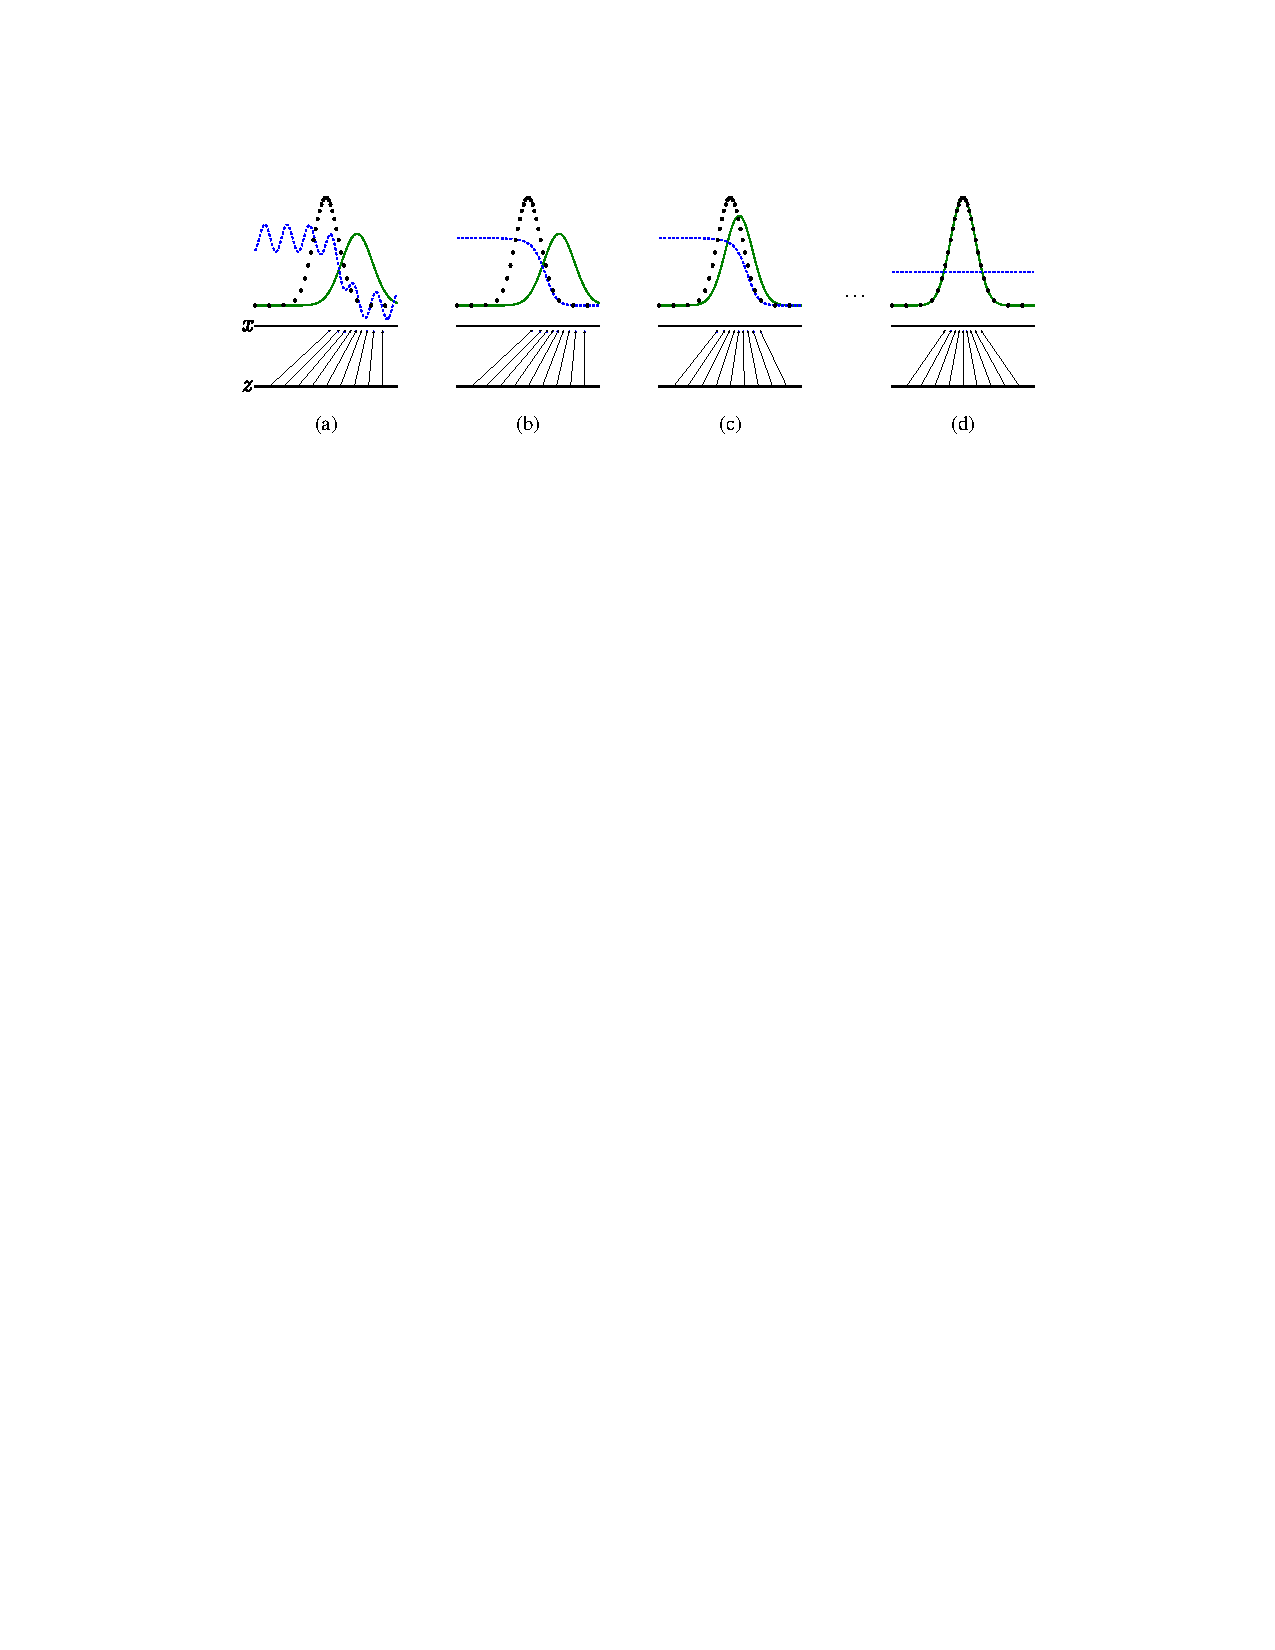
\includegraphics[width=1\textwidth]{GAN_training_vizualization.pdf}
  \caption{When optimizing GANs the discriminator and generator are optimized simultanously in an alternating procedure. The blue dashed line represents the discriminator probability of x belonging to the real data distribution rather than being created by the generator. The black dashed line represents the generative distribution and the green solid line the real data distribution. (a) shows a generator, discriminator pair near convergence, (b) shows the GAN performance after passing the inner loop of Algorithm \ref{alg.GAN_optimization}, which optimizes the discriminator. (c) shows the GAN performance after passing through one whole training loop in Algorithm \ref{alg.GAN_optimization}. Now the generator as well as the discriminator is optimized. (d) shows the GAN performance after several training iterations. The generator completely learned the data distribution, such that the discriminator is not able to separate between samples from the real data distribution and syntetics outputs of the generator \cite{Goodfellow2014}.}
  \label{fig:DCAN_model}
\end{figure}




\section{Deep belief network}

A Deep Belief Network(DBN) is a generative model that generates depth by stacking of Restricted Boltzmann machines (RBMs), which are widely used in research and application. Since DBMs are generative model they are used in an unsupervised or a supervised manner, which means, they are able to do feature learning/extraction and classification.

\subsection{Restricted Boltzmann machines}
RBMs consist of hidden and visible layers each containing several units. DBNs use Restricted Boltzmann machines (RBMs), which are a variation of regular Boltzmann machines with the restriction that it's units must form a bipartite graph. This requires that all RBM units are separated in two disjoint and independent subsets (hidden and visible subset). The visible and hidden units are connected through weighted connections but not the units belonging to the same layer. The units in the hidden and visible layer are binary. The matrix $W \in \mathbb{R}^{mxn}$ contains all the weights for connecting the m nodes of the hidden and n nodes of visible unit. $a \in \mathbb{R}^{m}$ and $b \in \mathbb{R}^{n}$ contains the biases of the hidden and visible unit \cite{Hinton2010}. The connection of the visible and hidden unit is visualized in \ref{fig:RBM}.

RBMs are Energy-based models, where for each combination of visible and hidden layer units $\mathbf{v,h}$ the following energy is calculated:

\begin{equation}
\begin{aligned}
    E(v,h) = -\sum_{i \in visible} a_{i}v_{i}-\sum_{j \in hidden} b_{j}h_{j}-\sum_{i,j} v_{i}h_{j}w_{ij},
\end{aligned}
\end{equation}
where $v_{i}$, $h_{j}$ are the binary states of the ith and jth unit in the visible and hidden layer. $a_{i}$, $b_{j}$ and $w_{ij}$ are the biases and weights corresponding to the ith unit in the visible and the jth unit in the hidden layer. Based on this energy the network assigns a probability to every possible combination of visible and hidden layer units:

\begin{equation}
\begin{aligned}
    p(\mathbf{v,h}) = \frac{1}{Z} e^{-E(\mathbf{v,h})},
\end{aligned}
\end{equation}
where Z is a "partition function". By summing over all possible combinations of hidden and visible layers the the probability $p(\mathbf{v,h})$ is normalized to a value between 0 and 1:

\begin{equation}
\begin{aligned}
    Z = \sum_{\mathbf{v,h}}e^{-E(\mathbf{v,h})}.
\end{aligned}
\end{equation}

The network assigns a probability for each training sample by summing $p(\mathbf{v,h})$ for all possible hidden vectors:
\begin{equation}
\begin{aligned}
    p(\mathbf{v}) = \frac{1}{Z} \sum_{h} e^{-E(\mathbf{v,h})}.
    \label{eq:prob_visible_layer}
\end{aligned}
\end{equation}

Since the units of RBMs must form a bipartite graph there are no connection between two hidden or visible units. Given a training sample the visible units can be calculated with eq. \ref{eq:prob_visible_layer}. From there the hidden units can be calculated as following:
\begin{equation}
\begin{aligned}
    P(v_{i}|h) = \sigma(a_{i} + \sum_{j=1}^{n} W_{i,j} h_{j}),
    \label{eq:prob_hidden_layer}
\end{aligned}
\end{equation}
where $h_{j}$ is the jth unit in the hidden layer and $v_{i}$ the ith unit in the visible layer. Afterwards the units of the visible layer can be reconstructed as following:
\begin{equation}
\begin{aligned}
    P(h_{i}|v) = \sigma(b_{j} + \sum_{i=1}^{n} W_{i,j} v_{i}).
    \label{eq:prob_reconstructed_visible_layer}
\end{aligned}
\end{equation}
This iterative RMB training is separated in two phases. The positive phase is the one where the hidden units are updated based on the visible units, which is defined in eq. \ref{eq:prob_hidden_layer}. The negative phase the visible units are updated based on the previously calculated hidden units, which is defined in eq. \ref{eq:prob_reconstructed_visible_layer}. This process is also visualized in fig. \ref{fig:RBM}. The weights and biases of the network can be updated such that the reconstruction error is minimized:

\begin{equation}
\begin{aligned}
    \Delta w_{ij} = \epsilon(\langle v_{i}, h_{j}\rangle_{data}- \langle v_{i}, h_{j}\rangle_{reconstructed}), 
    \label{eq:RBM_weight_update}
\end{aligned}
\end{equation}
where the angle brackets denote expectations under the distribution specified in the subscripts. The subscript $data$ refers to the expectation of the training set and subscript $reconstructed$ to the expectation of the defined model. A better training is achieved if more steps of alternating updating the visible and hidden layer are performed before collecting the statistics for the second term $\langle v_{i}, h_{j}\rangle_{reconstructed}$ in the learning rule \cite{Hinton2010}.

\begin{figure}[htpb]
  \centering
  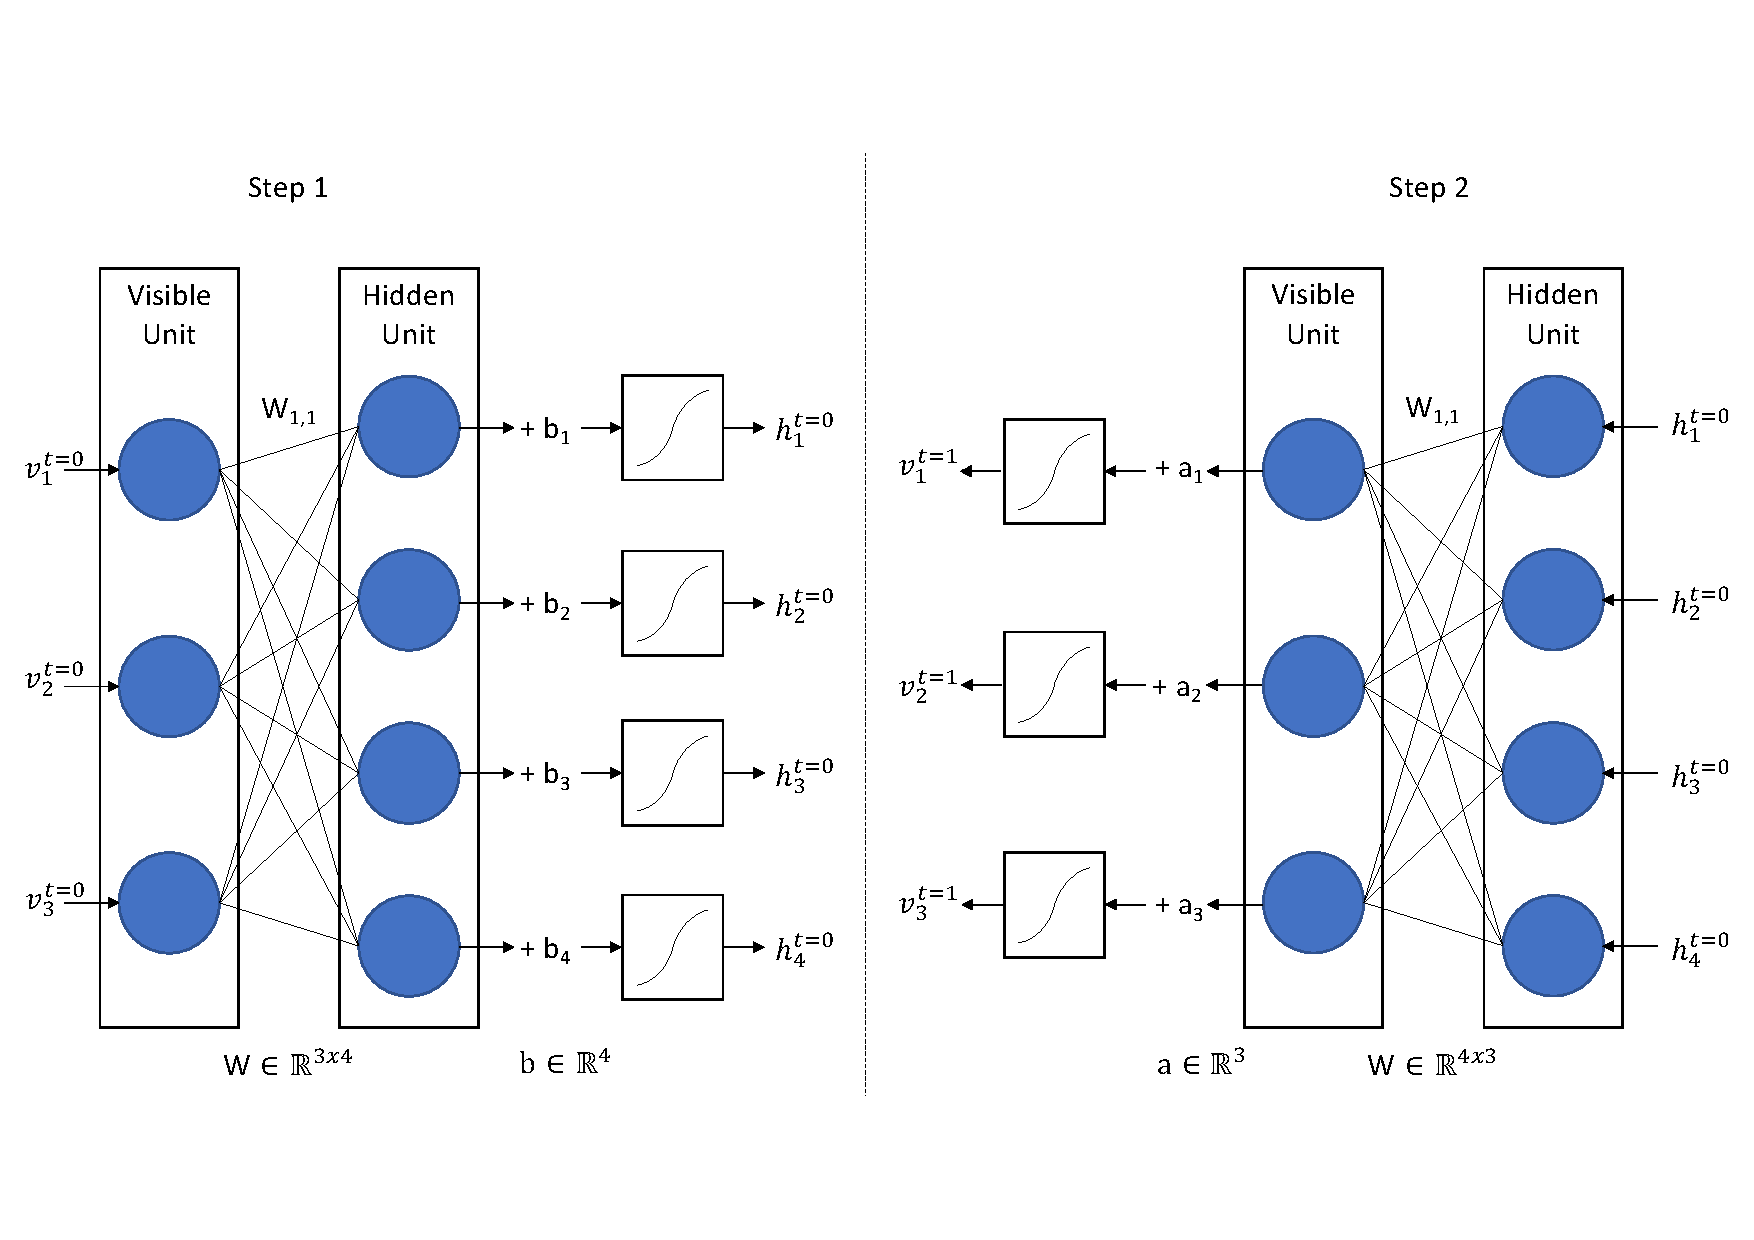
\includegraphics[width=1\textwidth]{RBM.pdf}
  \caption {Optimization of RBM} \label{fig:RBM}
\end{figure}
\FloatBarrier 

RBMs are generative models which make guesses about the probability distribution of the original input. By training the RBM the divergence between the true input distribution and the reconstructed ones is minimized \cite{Hinton2010}.

\subsection{Training Deep belief networks}
As shown in fig. \ref{fig:DBN} DBNs connect several RBMs in a specific order. The output of one RBM is used as input for the consecutive RBM. In a first step the units of the visible layer of the first RBM is calculated. Applying the positive and negative phase of the RBM training, the hidden visible layer of that RBM can be updated. The hidden layer of one RBM is treated as visible layer for the consecutive RBMs. This greedy learning algorithm is applied until all RBMs in the DBN are trained. After this layer to layer update is completed the supervised training of the DBN is started. The backpropagation training considers all layers simultanously while updating weights and biases in order to increase the classification accuracy of the DBN \cite{Zhang2017}.

\begin{figure}[htpb]
  \centering
  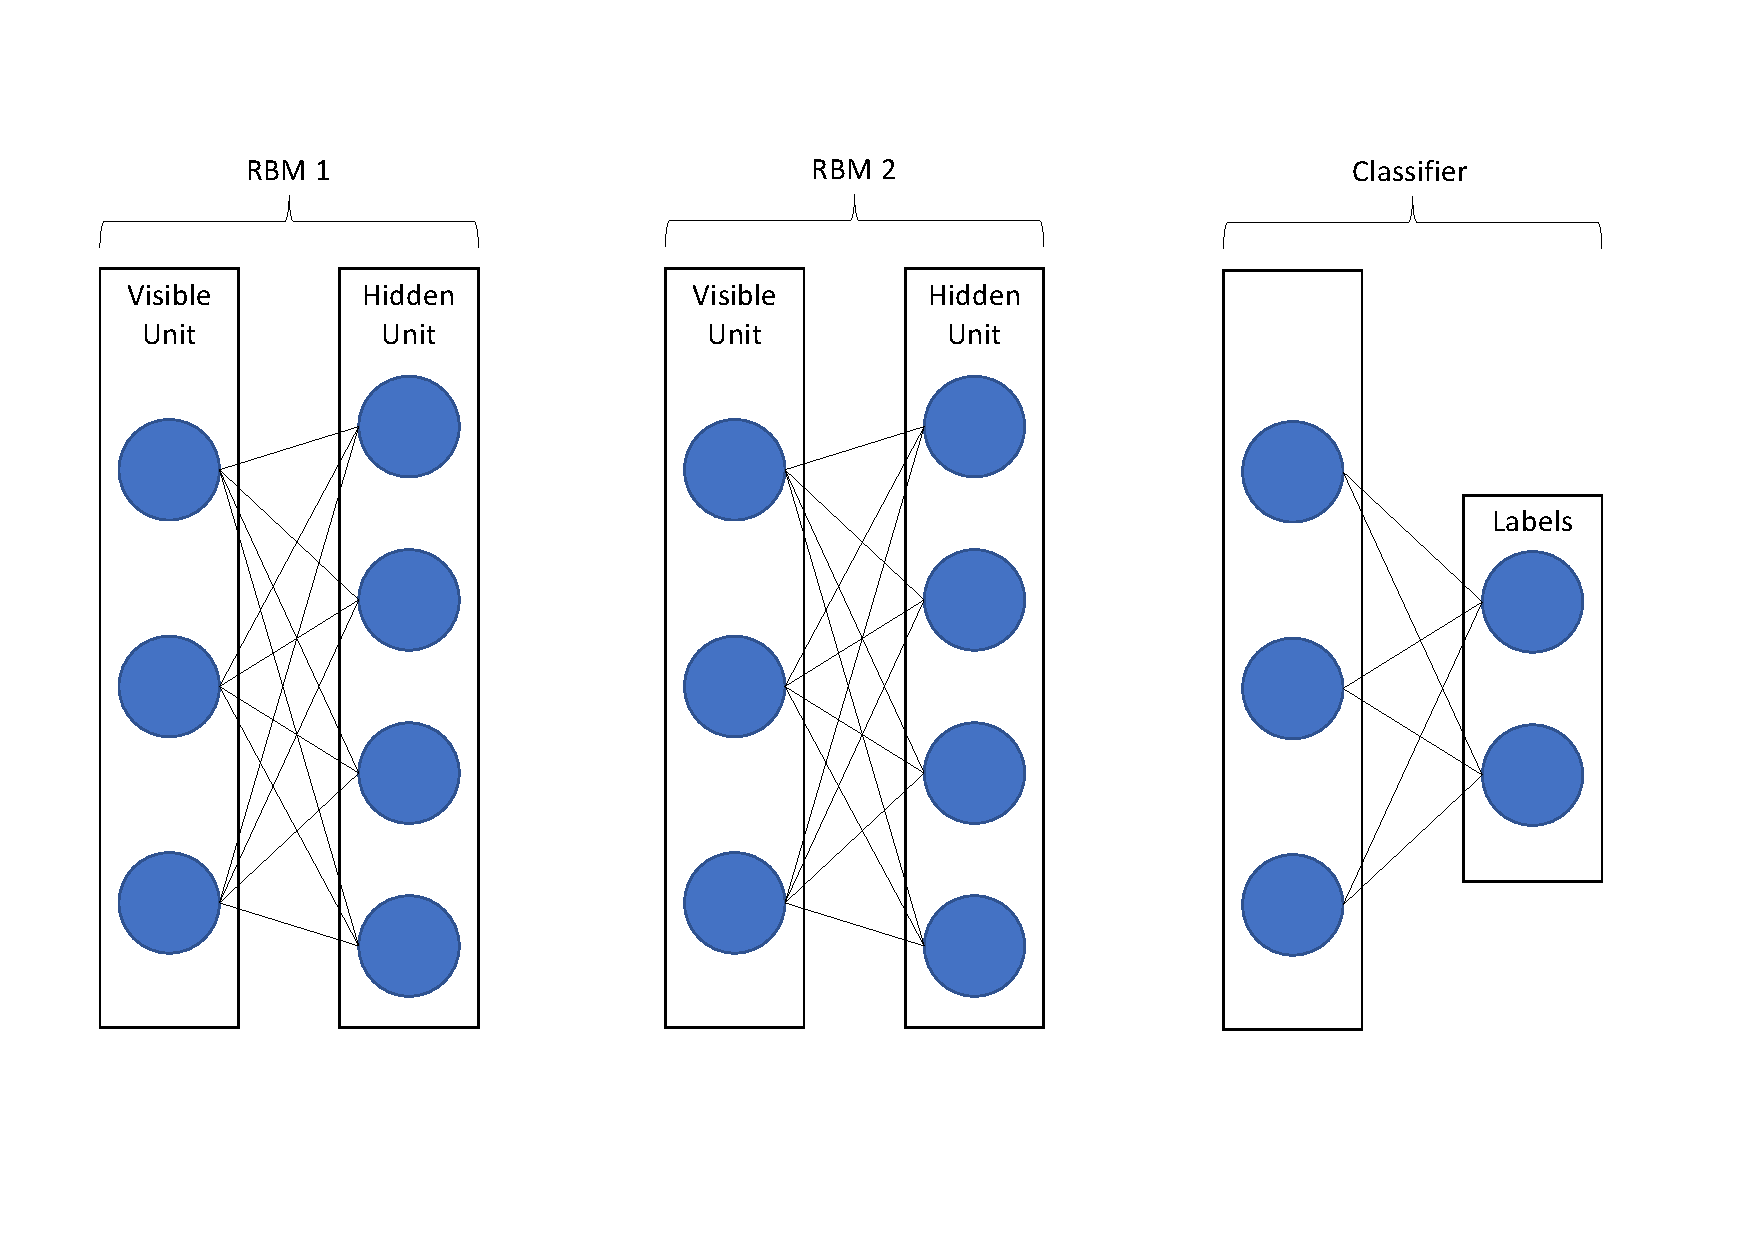
\includegraphics[width=1\textwidth]{DBN.pdf}
  \caption {Structure of DBN \cite{Zhang2017}} \label{fig:DBN}
\end{figure}
\FloatBarrier 

\section{Domain adaptation and Transfer Learning}

In the computer vision community domain adaption and transfer-learning techniques recently received more and more attention. In domain adaption a model is trained on the labeled training data, denoted as source domain. The model is then applied to solve an equal task on the unlabeled testing data, denoted as target domain. The target and source domain data come from different distributions, anyhow the data must be related in any sense and structured similarly. The conditional and marginal distribution for the source and target domain data differ. Transfer learning, also called multi-task learning, is related to domain adaption. The goal is to train a model solving a specific task on a given dataset. The model should then be used to solve a different task on the same data. For this reason the data distribution used for the two tasks has the same marginal distribution but different conditional distribution. This makes sense since the data used is equally distributed, but in different tasks relation between samples and labels will differ. In general one can say domain adaption is used to reduce the discrepancy between data distributions. This allows to train a model using the same task on data which is distributed differently. Transfer learning on the other hand learns a model, which is able to solve different tasks on the same data distribution. The differences are visualized in fig. \label{fig:domain_adaption_vs_transfer_learning}

\begin{figure}[htpb]
  \centering
  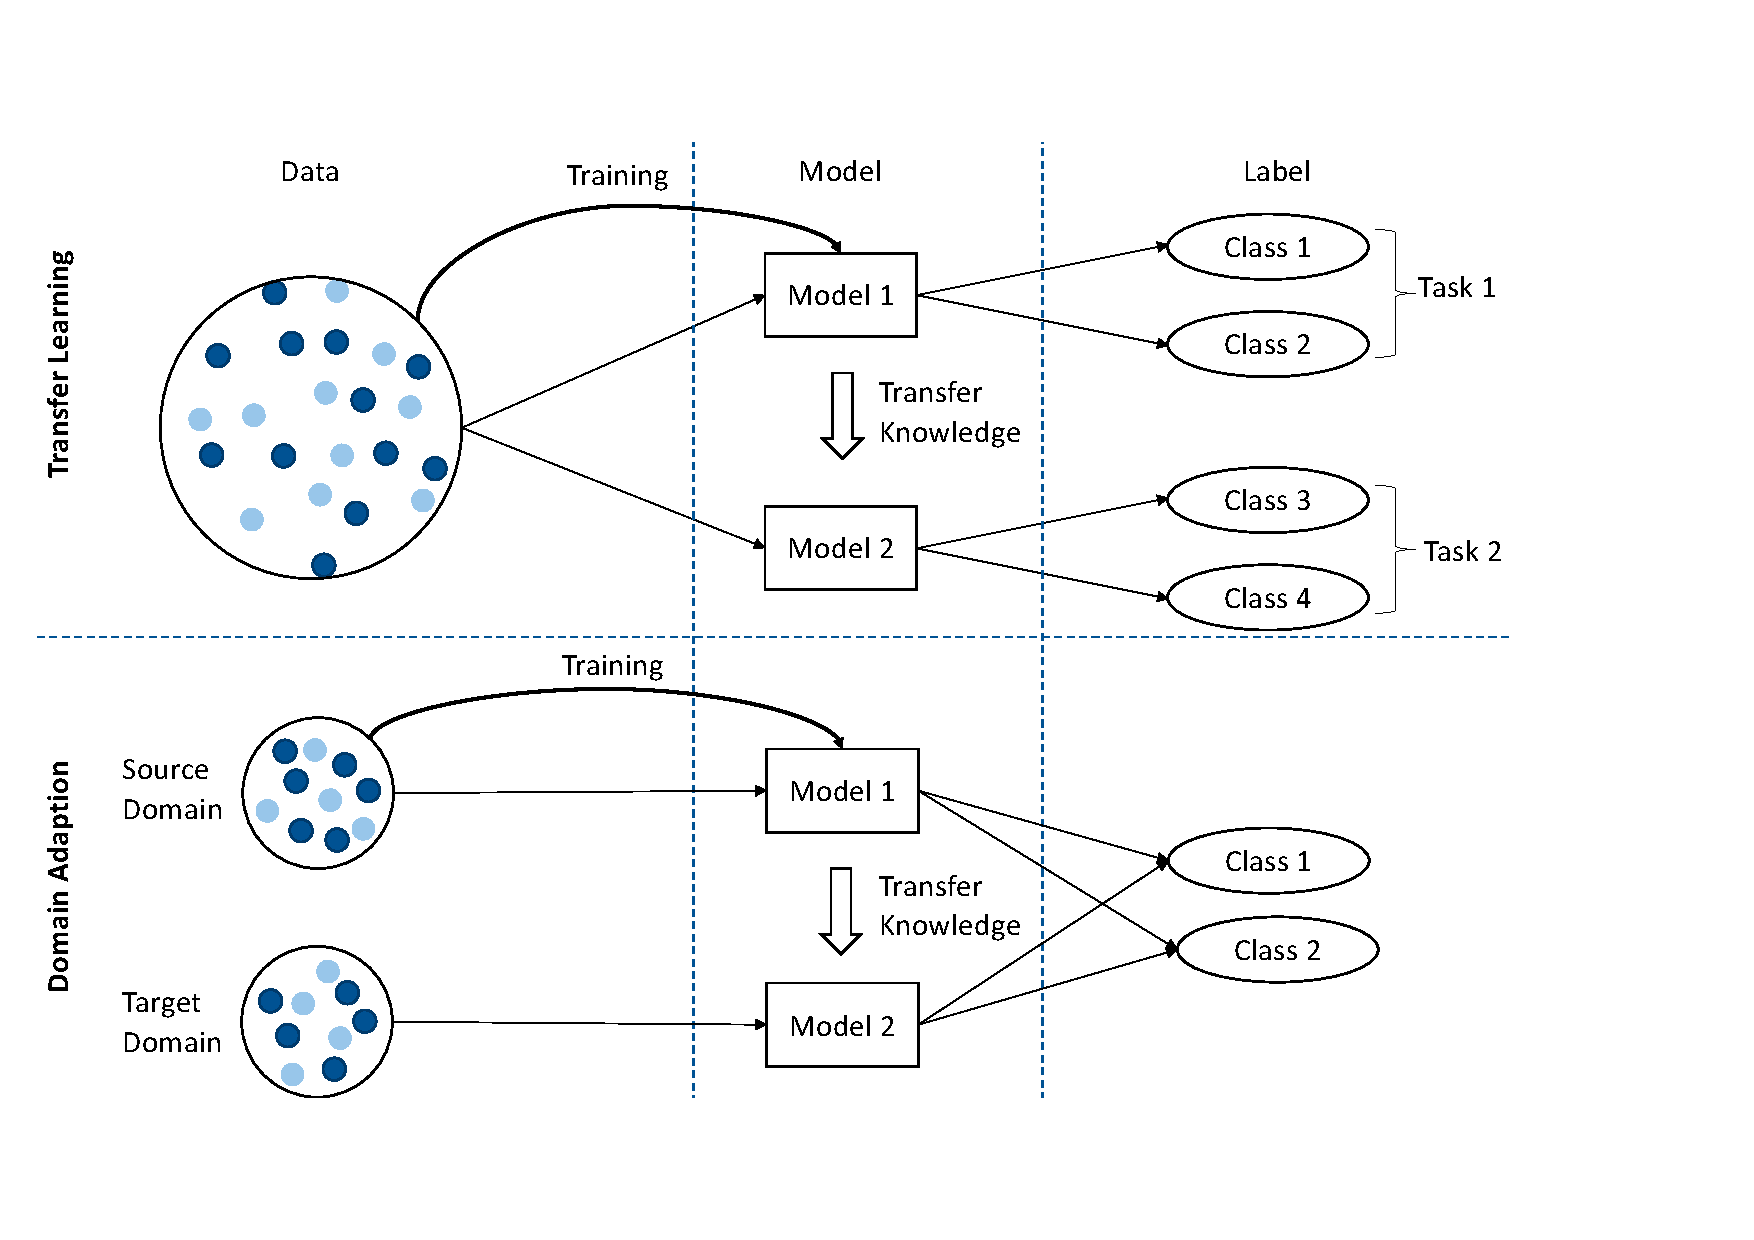
\includegraphics[width=.8\textwidth]{domain_adaption_vs_transfer_learning.pdf}
  \caption {Transfer Learning vs. Domain Adaption} \label{fig:domain_adaption_vs_transfer_learning}
\end{figure}
\FloatBarrier 

Since the focus of this thesis is to analyse domain adaption approaches the following passages are domain-adaption specific
\subsection{Notation}
The labeled source domain data is denoted by  $S = {(x_{i}^{s}, y_{i}^{s})_{i = 0}^{i = N_{s}}}$. Generally the target domain data is separated in labeled $T_{l} = {(x_{i}^{tl}, y_{i}^{tl})_{i = 0}^{i = N_{tl}}}$ and unlabeled data $T_{u} = {(x_{i}^{tu})_{i = 0}^{i = N_{tu}}}$. Usually it is assumed that there is a large amount of labeled data in the source and a small amount of labeled data in the target domain: $N_{tl} \ll N_{s}$. In this conext $x_{i}$ is referred as the observation and $y_{i}$ as the corresponding label  \cite{Patel2015}. Depending on the data available during training one differs between different branches of domain adaption \cite{Patel2015}: 
\begin{itemize}
\item \textbf{Semi-supervised domain adaptation}, where a function is learned using the data from $S$, $T_{l}$
\item \textbf{Unsupervised domain adaptation}, where a function is learned using the data from $S$ and $T_{u}$ 
\end{itemize}

From a statistical point of view the source and target domain can be described by the marginal distribution $P(X)$ and conditional distribution $P(Y|X)$. It is required that the data from source and target have the same data space and label space, while the marginal and conditional distribution differs $P(Y_{s}) \neq P(Y_{t})$ and $P(Y_{s}|X_{s}) \neq P(Y_{t}|X_{st})$ \cite{Qikang2020}

\subsection{Different types of transfer learning}
Generally domain adaption approaches can be grouped in four different types \cite{AZAMFAR2020103932}:  

\begin{itemize}
\item \textbf{Instance-based transfer learning} where different weights are assigned to data samples from the source domain. These weights are indicate the similarity between sample and target domain. When target and source domain samples show great similarity weights should be high such that those source samples are used preferably during training. This allows a training with source domain data which do not suffer that much from the domain discrepancy. 
\item \textbf{Feature-based transfer learning} which has the goal to find a feature space in which the discrepancy between domains is reduced. All source and target samples are transferred in the domain-invariant feature space where classification is easier. Fig.\ref{fig:Domain_adaption_intro} illustrates how feature-based domain adaption can be used to find a cross-domain classifier which accurately separates source and target domain data in a domain invariant feature space \cite{Pandhare2021}. 
\item \textbf{Model-based transfer learning} which uses classifiers that can be transferred directly or fine-tuned to make the model perform well on the target domain.
\item \textbf{Relation-based transfer learning} where the goal is to find and utilize similarities between the two domains to transfer knowledge. 
\end{itemize}


\begin{figure}[htpb]
  \centering
  \includegraphics[width=1\textwidth]{Domain_adaption_intro}
  \caption {Domain adaption for health monitoring of machines with different working conditions \cite{Pandhare2021}} \label{fig:Domain_adaption_intro}
\end{figure}
\FloatBarrier 



\section{Maximum Mean Discrepancy}
Maximum Mean Discrepancy (MMD) is a criterion which estimates the discrepancy between two distribution. MMD can be used to optimize the network such that the distribution discrepancy is reduced in a data domain-invariant feature space. The discrepancy is measured as squared distance between the distribution kernel embeddings in the reproducing kernel Hilbert space (RKHS). The distribution discrepancy across domains is measured in the layers of the neural network in order to avoid feature transferability degradation. One has to pay attention to not transfer noise or irrelevant information. This destroys the structure of the source and target domain data and therefore makes the classification task even more difficult \cite{li2020}. 

\begin{align}
    M_{k}(P,Q) = \Bigl|  \boldsymbol{E_{P}}[\Phi(\boldsymbol{X^{s}})] - \boldsymbol{E_{Q}}[\Phi(\boldsymbol{X^{t}})]     \Bigl|^{2}_{Hk}
\end{align}

Hk denotes the RKHS, which is described by the characteristic kernel k and the mapping function $\Phi$. Taking the identity function as mapping function results in matching the distribution means. When using more complex mapping functions also higher order moments can be matched \cite{Yujia2015}. The distributions of the source domain $X^{s} = \{{x}_{i}^{s}\}_{i=0,...,n_{s}}$ and target domain $X^{t} = \{{x}_{i}^{t}\}_{i=0,...,n_{t}}$ are represented by P and Q. $\boldsymbol{E_{p}[.]}$ is the expected value of the source distribution P in the feature space. The kernel choice is of great importance when applying MMD. For this reason it makes sense to combine several kernels in order to profit from their individual performance \cite{li2020}.

\begin{align}
    k(\boldsymbol{X^{s}}, \boldsymbol{X^{t}}) = \sum_{i=0}^{N_{k}} k_{\sigma_{i}}(\boldsymbol{X^{s}}, \boldsymbol{X^{t}})
\end{align}

$N_{k}$ denotes the number of kernels used in the the RKHS and $k_{\sigma_{i}}$ represents one individual RBF kernels. Also, other kernels like linear kernels could be used, but current research shows that RBF kernels usually perform best \cite{AZAMFAR2020103932}. In our attempt we used 5 RBF kernels with the bandwidth parameters 1, 2, 4, 8, 16.


